\chapter{HIỆN THỰC, ĐÁNH GIÁ VÀ THẢO LUẬN}\label{Chapter4}

\section*{Tóm tắt chương}

Chương này trình bày kế hoạch hiện thực và đánh giá hệ thống đề xuất. Nội dung bao gồm môi trường thí nghiệm, chuẩn bị dữ liệu, cấu hình chạy, chỉ số đánh giá, nhóm thí nghiệm và hướng thảo luận kết quả.

\section{Môi trường thực nghiệm}

\begin{itemize}
    \item \textbf{Máy 1}
    \begin{itemize}
        \item CPU: Intel\textregistered{} Core\texttrademark{} i9-13900k (16 cores - 2.9 GHz)
        \item GPU: NVIDIA GeForce\texttrademark{} RTX 3080 10GB LHR
        \item RAM: 22GB
        \item OS: Windows Subsystem for Linux 2 - Debian GNU/Linux 12
        \item Dung lượng ổ đĩa: 1TB
    \end{itemize}
    
    \item \textbf{Máy 2}
    \begin{itemize}
        \item CPU: AMD\textregistered{} Ryzen\texttrademark{} 9-5950X (16 cores - 3.4 Ghz)
        \item GPU: NVIDIA GeForce\texttrademark{} RTX 3090 24GB
        \item RAM: 32GB
        \item OS: Ubuntu GNU/Linux 20.04
        \item Dung lượng ổ đĩa: 870GB
    \end{itemize}

    \item \textbf{Môi trường phát triển}
    \begin{itemize}
        \item Trình soạn thảo: Visual Studio Code, OpenCode.
        \item Ngôn ngữ lập trình: Python3, Bash.
        \item Thư viện sử dụng: numpy, pandas, mathplotlib, sklearn, torch 2.12.0, pickle, cuda 13.2
    \end{itemize}
\end{itemize}

\section{Dữ liệu thực nghiệm}

Bộ dữ liệu được sử dụng trong nghiên cứu này là CICIoT2023 \cite{ciciot2023}, một tập dữ liệu phát hiện xâm nhập quy mô lớn được thu thập trên hạ tầng thiết bị IoT thực tế, trong đó lưu lượng bình thường được ghi nhận song song với nhiều họ tấn công khác nhau nhằm phản ánh sát thực tế vận hành của một hệ thống IDS. Trước khi đưa vào huấn luyện, dữ liệu thô được làm sạch qua bước tiền xử lý, trong đó các bản ghi mang giá trị rỗng, giá trị vô cực hoặc bản ghi trùng lặp đều được loại bỏ, đồng thời các đặc trưng số được chuẩn hoá về cùng một thang đo để tránh việc một vài đặc trưng có biên độ lớn lấn át quá trình học. Sau bước chuẩn hoá, mỗi luồng mạng được biểu diễn bằng một vector đặc trưng $20$ chiều, trong đó $20$ cột đầu đóng vai trò là đầu vào của mô hình còn cột cuối cùng lưu nhãn lớp tương ứng.

Tập đặc trưng $20$ chiều bao quát nhiều khía cạnh của một luồng mạng, từ đặc tính thời gian, kích thước và thống kê gói, đến các cờ giao thức TCP cùng tỉ lệ phân bố giao thức. Bảng \ref{tab:cic23_features} liệt kê đầy đủ $20$ đặc trưng, được nhóm lại theo bản chất nhằm thuận tiện cho phần thảo luận sau này. Việc giới hạn ở $20$ đặc trưng giúp giảm chi phí huấn luyện trong mô phỏng nhiều client, đồng thời vẫn bảo toàn các tín hiệu quan trọng để phân biệt lưu lượng bình thường với các nhóm tấn công, vốn thường khác nhau ở mặt kích thước gói, tần suất truyền và phân bố cờ TCP.

\begin{table}[H]
    \centering
    \caption{Tập $20$ đặc trưng đầu vào của CICIoT2023.}
    \label{tab:cic23_features}
    \begin{tabular}{lp{0.62\linewidth}}
        \hline
        Nhóm đặc trưng & Tên đặc trưng \\
        \hline
        Thời gian luồng       & flow\_duration, IAT \\
        Kích thước gói        & Tot size, Tot sum, AVG, Min, Max, Magnitue, Header\_Length \\
        Cờ TCP (xuất hiện)    & syn\_flag\_number, ack\_flag\_number, psh\_flag\_number, rst\_flag\_number, fin\_flag\_number \\
        Số đếm cờ TCP            & syn\_count, ack\_count, rst\_count \\
        Tỉ lệ giao thức       & TCP, UDP, ICMP \\
        \hline
    \end{tabular}
\end{table}

Tập dữ liệu sau tiền xử lý chứa $46{,}905{,}384$ bản ghi trải trên $34$ lớp, gồm một lớp lưu lượng bình thường (BenignTraffic) và $33$ lớp tấn công thuộc nhiều nhóm khác nhau. Các lớp tấn công này được tổ chức thành những nhóm lớn, bao gồm nhóm tấn công từ chối dịch vụ phân tán (DDoS) với nhiều biến thể như DDoS-ICMP\_Flood, DDoS-SYN\_Flood hay DDoS-UDP\_Flood, nhóm tấn công từ chối dịch vụ (DoS), họ mã độc Mirai, nhóm trinh sát (Recon), nhóm giả mạo như DNS\_Spoofing và MITM-ArpSpoofing, nhóm tấn công tầng web như XSS, SqlInjection và CommandInjection, cùng nhóm dò mật khẩu DictionaryBruteForce.

Một đặc điểm nổi bật của CICIoT2023 là phân phối lớp mất cân bằng nghiêm trọng, điều vốn phản ánh đúng bản chất của dữ liệu an ninh mạng, nơi một số kiểu tấn công xuất hiện với tần suất rất cao trong khi nhiều kiểu khác lại hiếm gặp. Bảng \ref{tab:cic23_dist} liệt kê toàn bộ $34$ lớp cùng số mẫu và tỉ lệ tương ứng trên toàn tập dữ liệu, được sắp xếp theo thứ tự giảm dần của số mẫu. Lớp đa số DDoS-ICMP\_Flood chiếm tới $15.42\%$ tổng số bản ghi, gấp khoảng $5{,}750$ lần so với lớp Uploading\_Attack vốn chỉ có $1{,}257$ mẫu. Mười lớp giàu mẫu nhất, đều thuộc nhóm DDoS hoặc DoS, đã chiếm hơn $90\%$ toàn tập, trong khi $24$ lớp còn lại chia nhau chưa tới $10\%$. Sự chênh lệch hàng nghìn lần giữa lớp giàu nhất và lớp nghèo nhất khiến cho việc phát hiện các lớp thiểu số trở thành thách thức trọng tâm, đặc biệt khi dữ liệu lại tiếp tục bị phân mảnh và lệch nhãn trong môi trường học liên kết.

\begin{table}[H]
    \centering
    \caption{Phân phối toàn bộ $34$ lớp trong CICIoT2023, sắp xếp giảm dần theo số mẫu.}
    \label{tab:cic23_dist}
    \small
    \begin{tabular}{rlrr}
        \hline
        ID & Lớp & Số mẫu & \% \\
        \hline
        6  & DDoS-ICMP\_Flood          & 7{,}234{,}033 & 15.42 \\
        4  & DDoS-UDP\_Flood           & 5{,}437{,}630 & 11.59 \\
        5  & DDoS-TCP\_Flood           & 4{,}518{,}631 & 9.63 \\
        2  & DDoS-PSHACK\_Flood        & 4{,}114{,}128 & 8.77 \\
        3  & DDoS-SYN\_Flood           & 4{,}078{,}425 & 8.70 \\
        1  & DDoS-RSTFINFlood          & 4{,}064{,}317 & 8.66 \\
        7  & DDoS-SynonymousIP\_Flood  & 3{,}614{,}936 & 7.71 \\
        13 & DoS-UDP\_Flood            & 3{,}334{,}095 & 7.11 \\
        15 & DoS-TCP\_Flood            & 2{,}683{,}771 & 5.72 \\
        14 & DoS-SYN\_Flood            & 2{,}038{,}148 & 4.35 \\
        0  & BenignTraffic             & 1{,}103{,}395 & 2.35 \\
        17 & Mirai-greeth\_flood       & 996{,}594     & 2.12 \\
        19 & Mirai-udpplain            & 894{,}884     & 1.91 \\
        18 & Mirai-greip\_flood        & 755{,}288     & 1.61 \\
        10 & DDoS-ICMP\_Fragmentation  & 454{,}621     & 0.97 \\
        26 & MITM-ArpSpoofing          & 309{,}025     & 0.66 \\
        9  & DDoS-UDP\_Fragmentation   & 288{,}317     & 0.61 \\
        8  & DDoS-ACK\_Fragmentation   & 286{,}488     & 0.61 \\
        25 & DNS\_Spoofing             & 179{,}738     & 0.38 \\
        24 & Recon-HostDiscovery       & 135{,}030     & 0.29 \\
        21 & Recon-OSScan              & 98{,}684      & 0.21 \\
        22 & Recon-PortScan            & 82{,}683      & 0.18 \\
        16 & DoS-HTTP\_Flood           & 72{,}211      & 0.15 \\
        23 & VulnerabilityScan         & 37{,}525      & 0.08 \\
        12 & DDoS-HTTP\_Flood          & 28{,}917      & 0.06 \\
        11 & DDoS-SlowLoris            & 23{,}526      & 0.05 \\
        33 & DictionaryBruteForce      & 13{,}121      & 0.03 \\
        27 & BrowserHijacking          & 5{,}889       & 0.01 \\
        32 & CommandInjection          & 5{,}435       & 0.01 \\
        31 & SqlInjection              & 5{,}272       & 0.01 \\
        29 & XSS                       & 3{,}862       & 0.01 \\
        28 & Backdoor\_Malware         & 3{,}236       & 0.01 \\
        20 & Recon-PingSweep           & 2{,}272       & 0.00 \\
        30 & Uploading\_Attack         & 1{,}257       & 0.00 \\
        \hline
    \end{tabular}
\end{table}

Toàn bộ tập dữ liệu sau tiền xử lý được phân hoạch cho client theo ngữ cảnh Non-IID, đồng thời một tập kiểm thử toàn cục được giữ cố định và dùng chung cho mọi thuật toán nhằm bảo đảm việc so sánh diễn ra trên cùng một thước đo. Tập kiểm thử này được tách theo phân tầng giữ nguyên tỉ lệ lớp, nên phân phối nhãn trên tập kiểm thử trùng khớp với phân phối trên toàn tập, qua đó các lớp thiểu số vẫn hiện diện đầy đủ trong quá trình đánh giá.

Sau khi dữ liệu được tách theo lớp, mỗi lớp được phân bổ cho client theo ngữ cảnh Non-IID lệch nhãn (label skew), trong đó số mẫu của một lớp trên các client được lấy từ phân phối Dirichlet:
\[
\pi_c\sim \operatorname{Dir}(\alpha\mathbf{1}_{|K|}),
\qquad
n_{k,c}=\left\lfloor \pi_{k,c}N_c\right\rfloor,
\]
trong đó $N_c$ là số mẫu của lớp $c$, $|K|$ là số client và $n_{k,c}$ là số mẫu lớp $c$ được cấp cho client $k$. Vì phép lấy mẫu được lặp lại độc lập cho từng lớp, một client có thể giàu dữ liệu ở vài lớp nhưng thiếu nghiêm trọng ở các lớp khác, phản ánh tình huống IDS trong đó mỗi tổ chức chỉ quan sát một phần của không gian tấn công. Tham số $\alpha$ điều khiển mức độ lệch nhãn, và giá trị cụ thể được lựa chọn cho từng kịch bản thực nghiệm sẽ được trình bày ở phần sau. Phân phối thu được khi $\alpha=0.1$ được minh họa trong hình \ref{fig:partition}.

\section{Kịch bản thực nghiệm}

Nghiên cứu này được tiến hành nhằm đánh giá và so sánh năng lực của các phương pháp học tiệm tiến theo lớp khi vận hành trong điều kiện hệ thống phát hiện xâm nhập phải liên tục mở rộng theo thời gian. Quá trình thực nghiệm đặt phương pháp đề xuất bên cạnh một tập rộng các phương pháp học tiệm tiến tiêu biểu, được phân thành ba nhóm chính, bao gồm nhóm dựa trên ràng buộc tham số (EWC, MAS, LwF, PASS, CBKD EFCIL), nhóm dựa trên học tái diễn (iCaRL, BiC) và nhóm dựa trên kiến trúc động (FOSTER); ngoài ra, một cấu hình học liên kết không có cơ chế tiệm tiến (fine tuning) cũng được giữ lại làm cận dưới để làm nổi bật mức độ quên thảm khốc khi không áp dụng bất kỳ biện pháp giữ tri thức nào. Mục tiêu chính của quá trình so sánh là làm rõ khả năng của từng phương pháp trong việc tiếp nhận các lớp tấn công mới mà vẫn duy trì tri thức đã học, đồng thời quan sát chi phí truyền thông mà mỗi phương pháp phải gánh chịu trong từng vòng trao đổi.

Để phản ánh sát thực tế triển khai, toàn bộ hệ thống được thiết kế với $100$ client, trong đó dữ liệu của các client được chia thành $7$ task học tiệm tiến nối tiếp nhau. Mỗi task trong quá trình huấn luyện được gắn với một nhóm lớp tấn công mới hoàn toàn chưa từng xuất hiện ở các task trước, đồng thời cũng đi kèm một nhóm client mới gia nhập hệ thống. Cách tổ chức này được lựa chọn nhằm mô phỏng tình huống trong đó mạng lưới IDS liên kết được mở rộng dần qua thời gian, vừa do số lượng tổ chức tham gia tăng lên, vừa do không gian tấn công mà hệ thống phải nhận diện ngày càng phong phú. Trong mọi task, dữ liệu của nhóm client đang hoạt động được phân hoạch lại theo phân phối Dirichlet với tham số $\alpha=0.1$, qua đó tái tạo ngữ cảnh Non-IID lệch nhãn nghiêm trọng, nơi mỗi client chỉ quan sát được một phần nhỏ của không gian tấn công.

Số lượng client tham gia được thiết kế tăng dần theo từng task nhằm mô phỏng quá trình các tổ chức mới lần lượt gia nhập hệ thống IDS liên kết. Ở task đầu tiên, chỉ có $40$ client tham gia huấn luyện; sau đó, mỗi task tiếp theo bổ sung thêm $10$ client, cho đến khi task cuối cùng quy tụ toàn bộ $100$ client của hệ thống. Bảng \ref{tab:cil_client_growth} tóm tắt số lượng client tích luỹ cùng số client mới gia nhập ở từng task, qua đó cho thấy quá trình mở rộng quy mô của hệ thống diễn ra đều đặn theo thời gian.

\begin{table}[H]
    \centering
    \caption{Số lượng client theo từng task trong kịch bản học tiệm tiến.}
    \label{tab:cil_client_growth}
    \begin{tabular}{cccc}
        \hline
        Task & Client tích luỹ & Client mới & Tỉ lệ (\%) \\
        \hline
        0 & 40  & 40 & 40\% \\
        1 & 50  & 10 & 50\% \\
        2 & 60  & 10 & 60\% \\
        3 & 70  & 10 & 70\% \\
        4 & 80  & 10 & 80\% \\
        5 & 90  & 10 & 90\% \\
        6 & 100 & 10 & 100\% \\
        \hline
    \end{tabular}
\end{table}

Song song với quá trình mở rộng số lượng client, không gian lớp tấn công mà hệ thống phải xử lý cũng được mở rộng theo từng task. Toàn bộ $34$ lớp của tập dữ liệu được phân bổ vào bảy task, trong đó sáu task đầu mỗi task tiếp nhận $5$ lớp mới, còn task cuối cùng tiếp nhận $4$ lớp còn lại. Bảng \ref{tab:cil_task_classes} trình bày chi tiết phân bổ lớp theo từng task, cho thấy mỗi task đều đưa vào hệ thống một tập lớp hoàn toàn mới mà các phương pháp học tiệm tiến phải tiếp nhận mà không được quên tri thức đã tích luỹ từ những task trước. Lớp Benign được cố định ở task đầu tiên, trong khi các lớp tấn công còn lại hoàn toàn được chọn ngẫu nhiên cho từng task.

\begin{table}[H]
    \centering
    \caption{Phân bổ lớp theo từng task trong kịch bản học tiệm tiến.}
    \label{tab:cil_task_classes}
    \small
    \begin{tabular}{clc}
        \hline
        Task & Các lớp trong task & Số lớp \\
        \hline
        0 & BenignTraffic, DictionaryBruteForce, DoS-HTTP\_Flood, & 5 \\
          & BrowserHijacking, Mirai-greip\_flood & \\
        1 & DDoS-UDP\_Fragmentation, DDoS-ICMP\_Fragmentation, & 5 \\
          & Recon-PingSweep, Recon-PortScan, DoS-UDP\_Flood & \\
        2 & DDoS-RSTFINFlood, DDoS-TCP\_Flood, Mirai-greeth\_flood, & 5 \\
          & DDoS-ICMP\_Flood, DoS-SYN\_Flood & \\
        3 & DDoS-HTTP\_Flood, DNS\_Spoofing, DDoS-PSHACK\_Flood, & 5 \\
          & DDoS-SYN\_Flood, Uploading\_Attack & \\
        4 & DDoS-UDP\_Flood, Backdoor\_Malware, Recon-HostDiscovery, & 5 \\
          & SqlInjection, VulnerabilityScan & \\
        5 & Mirai-udpplain, MITM-ArpSpoofing, DDoS-SynonymousIP\_Flood, & 5 \\
          & Recon-OSScan, DictionaryBruteForce & \\
        6 & DDoS-ACK\_Fragmentation, DDoS-SlowLoris, DoS-TCP\_Flood, XSS & 4 \\
        \hline
        \multicolumn{2}{l}{Tổng cộng} & 34 \\
        \hline
    \end{tabular}
\end{table}

Để bảo đảm mỗi client nhận đủ dữ liệu huấn luyện, dữ liệu của từng task được phân hoạch lại hoàn toàn từ đầu chỉ cho nhóm client đang tích cực tham gia task đó. Cách tiếp cận này khác với kịch bản học liên kết thông thường, nơi toàn bộ $100$ client nhận phân hoạch cố định từ đầu; thay vào đó, phân hoạch được tái tạo cho từng task dựa trên số client tham gia lúc đó, qua đó phản ánh đúng tình huống mở rộng mạng lưới liên kết theo thời gian. Sau khi phân hoạch, một tỉ lệ ngẫu nhiên trong khoảng $[5\%, 20\%]$ số mẫu của từng client được tách ra làm phần dữ liệu công khai, phần còn lại giữ làm dữ liệu riêng. Vì tỉ lệ cắt được lấy độc lập cho mỗi client, tổng phần công khai trên toàn hệ thống là $7{,}935{,}448$ mẫu ($16.92\%$), còn $38{,}969{,}936$ mẫu ($83.08\%$) được giữ làm dữ liệu riêng cho huấn luyện giám sát cục bộ.

\begin{figure*}[ht]
    \centering
    
\includegraphics[width=1.0\textwidth]{images/partition.png}
    \caption{Phân phối dữ liệu theo lớp cho 100 client.}
\label{fig:partition}
\end{figure*}

Bên cạnh kịch bản chuẩn trong đó mọi client cùng dùng một loại kiến trúc, đề tài này còn xây dựng thêm một kịch bản mô hình hỗn hợp (mixed model architectures, kí hiệu multiple) nhằm kiểm chứng tính linh hoạt của kỹ thuật học chắt lọc liên kết trong phương pháp đề xuất. Trong kịch bản hỗn hợp, các client trong hệ thống được phép sử dụng những kiến trúc mạng khác nhau thay vì bị ràng buộc chung một mô hình, qua đó phản ánh tình huống thực tế nơi mỗi tổ chức tự lựa chọn cấu hình phù hợp với hạ tầng riêng. Quá trình trao đổi tri thức giữa các client lúc này không còn dựa trên việc tổng hợp trọng số, mà chuyển sang trao đổi logits trên tập dữ liệu công khai, nhờ đó hệ thống vẫn có thể phối hợp học tập dù mỗi client mang một mô hình khác biệt về cấu trúc.

% Trước khi đi vào kết quả, chi phí truyền thông của từng phương pháp cũng được ước lượng ở mức một client trong một vòng huấn luyện, với giả định mọi tensor số thực dùng định dạng float32 và nhãn cứng dùng int64. Theo hiện thực trong mã nguồn, FedAvg truyền trọng số mô hình cùng một số vô hướng biểu diễn kích thước dữ liệu client; GLFC giữ cơ chế FedAvg nhưng bổ sung các gradient của encoder dùng cho proxy server; FEAT thay tầng phân loại cuối bằng ETF cố định nên không cần truyền trọng số của tầng logits, đồng thời chỉ gửi thêm hai đại lượng năng lượng head--tail; còn phương pháp đề xuất truyền logits trên tập công khai, mặt nạ nhị phân tương ứng và nhận lại logits đồng thuận cùng nhãn giả cứng. Với $C=34$, mô hình có khoảng $259{,}810$ tham số, phần mô hình không tính tầng ETF của FEAT có khoảng $257{,}600$ tham số, encoder của GLFC có khoảng $32{,}258$ tham số, và số mẫu công khai trung bình mỗi task được xấp xỉ bởi $P=7{,}935{,}448/7\approx1.13$ triệu mẫu.

% \begin{table}[H]
%     \centering
%     \caption{Ước lượng chi phí truyền thông mỗi client trong một vòng huấn luyện.}
%     \label{tab:comm_cost_cil}
%     \resizebox{\linewidth}{!}{
%     \begin{tabular}{lcccccc}
%         \hline
%         \multirow{2}{*}{Phương pháp} & \multicolumn{2}{c}{Lý thuyết} & \multicolumn{2}{c}{Thực tế} & \multirow{2}{*}{Tổng} \\
%         \cline{2-5}
%         & Upload & Download & Upload & Download & \\
%         \hline
%         FedAvg & $|\theta|+1$ & $|\theta|$ & $1.04$ MB & $1.04$ MB & $2.08$ MB \\
%         GLFC & $|\theta|+1+G_{\mathrm{enc}}$ & $|\theta|$ & $3.50$ MB & $1.16$ MB & $4.66$ MB \\
%         FEAT & $|\theta|-|\theta_{\mathrm{logits}}|+2$ & $|\theta|-|\theta_{\mathrm{logits}}|$ & $1.03$ MB & $1.03$ MB & $2.06$ MB \\
%         Đề xuất & $(P+E)C$ logits $+(P+E)C$ mask & $(P+E)C$ logits $+(P+E)$ nhãn & $200$ MB & $155.96$ MB & $355.96$ MB \\
%         \hline
%     \end{tabular}}
% \end{table}

% Trong bảng \ref{tab:comm_cost_cil}, $G_{\mathrm{enc}}$ được tính theo giới hạn tối đa $20$ bộ gradient encoder mà GLFC lưu trong \texttt{proto\_grad\_pool}, nên phần phụ trội xấp xỉ $20\times32{,}258\times4=2.58$ MB. Với phương pháp đề xuất, $E$ biểu diễn số mẫu replay từ các task cũ; do cấu hình mặc định giữ khoảng $1\%$ mẫu công khai theo từng lớp, phần này nhỏ hơn nhiều so với $P$ và được gộp vào ước lượng cuối. Vì vậy, phương pháp đề xuất có chi phí lớn hơn ở từng vòng trao đổi, nhưng phần truyền thông này là logits trên dữ liệu công khai và exemplar thay vì trọng số mô hình riêng của client.

\section{Thiết lập thực nghiệm}

\subsection{Cấu hình huấn luyện chung}

Các mô hình chính trong thí nghiệm được hiện thực bằng PyTorch. Đầu vào của mỗi mô hình là vector đặc trưng $x\in\mathbb{R}^{20}$, còn đầu ra là vector logits có kích thước bằng số lớp hiện tại. Trong chế độ dự đoán, logits được đưa qua hàm softmax để tạo phân phối xác suất; trong huấn luyện, loss được tính trực tiếp trên logits để giữ ổn định số học.

Tất cả các mô hình phân loại dùng Adam làm bộ tối ưu. Learning rate mặc định được co giãn theo batch size:
\[
\eta=10^{-3}\sqrt{\frac{B}{1024}},
\]
trong đó $B$ là batch size. Batch size mặc định là $8192$. Learning rate dùng warm-up tuyến tính:
\[
\eta_e= \eta\frac{e+1}{5}
\]
Hàm mất mát cho học giám sát là cross-entropy với label smoothing $0.05$. Gradient được chuẩn hoá bằng clipping theo chuẩn $\ell_2$ với ngưỡng $0.5$. Một số lớp tuyến tính được áp dụng weight decay $10^{-4}$ để giảm overfitting, trong khi các tham số còn lại không dùng weight decay. Các mô hình dùng LayerNorm thay cho BatchNorm vì thí nghiệm có batch lớn, dữ liệu Non-IID và phân phối giữa client khác nhau; LayerNorm giúp chuẩn hoá biểu diễn theo từng mẫu và ít phụ thuộc thống kê batch hơn.

\subsection{Mô hình GRU}
\label{sec:gru_arch}

GRU \cite{kasongo2023gru} xử lý vector 20 chiều như chuỗi một chiều có độ dài 20, mỗi bước thời gian chứa một giá trị đặc trưng. Cách biểu diễn này cho phép mô hình học quan hệ tuần tự tương đối giữa các đặc trưng sau tiền xử lý, đồng thời vẫn giữ chi phí thấp hơn BiLSTM. Bảng \ref{tab:gru_arch} trình bày kiến trúc GRU.

\begin{table}[H]
\centering
\caption{Kiến trúc GRU dùng trong thí nghiệm.}
\label{tab:gru_arch}
\begin{tabular}{lll}
\hline
Tầng & Kích thước & Thiết lập \\
\hline
Reshape & $20\rightarrow20\times1$ & Mỗi đặc trưng là một bước chuỗi \\
GRU 1 & $1\rightarrow128$ & Trả về toàn bộ chuỗi, LayerNorm, Dropout $0.15$ \\
GRU 2 & $128\rightarrow128$ & Trả về toàn bộ chuỗi, LayerNorm, Dropout $0.15$ \\
GRU 3 & $128\rightarrow128$ & Lấy trạng thái cuối, LayerNorm, Dropout $0.15$ \\
Dense head & $128\rightarrow64$ & ReLU, LayerNorm, Dropout $0.20$ \\
Classifier & $64\rightarrow C$ & Logits theo số lớp $C$ \\
\hline
\end{tabular}
\end{table}

Ba tầng GRU liên tiếp cho phép mô hình tích luỹ tương tác phi tuyến giữa các đặc trưng. Hai tầng đầu giữ toàn bộ chuỗi để tầng sau tiếp tục xử lý thông tin theo vị trí đặc trưng, còn tầng cuối chỉ lấy trạng thái cuối làm biểu diễn toàn cục. Dense head dùng ReLU vì đây là tầng nén cuối trước logits, cần ánh xạ rõ ràng và gọn hơn thay vì giữ dạng kích hoạt trơn như MLP. Weight decay chỉ áp dụng lên tầng head, còn các tầng GRU không dùng weight decay để tránh làm yếu khả năng ghi nhớ trong các cổng cập nhật.

Mô hình GRU được sử dụng cho kịch bản đơn kiến trúc để so sánh với các kịch bản học tiệm tiến dựa trên thuật toán FedAvg.

\subsection{Mô hình DCNN--BiLSTM}
\label{sec:dcblstm_arch}
DCNN--BiLSTM \cite{hnamte2023dcnnbilstm} là mô hình sâu hơn, kết hợp trích xuất mẫu cục bộ bằng tích chập một chiều và mô hình hoá phụ thuộc hai chiều bằng BiLSTM. Bảng \ref{tab:dcblstm_arch} mô tả kiến trúc của mô hình này.

\begin{table}[H]
\centering
\caption{Kiến trúc CNN--BiLSTM dùng trong thí nghiệm.}
\label{tab:dcblstm_arch}
\begin{tabular}{lll}
\hline
Tầng & Kích thước & Thiết lập \\
\hline
Reshape & $20\rightarrow1\times20$ & Một kênh đầu vào \\
Conv1D & $1\rightarrow64$ & Kernel size $20$, padding same, ReLU, LayerNorm \\
BiLSTM 1 & $64\rightarrow2\times64$ & Trả về toàn bộ chuỗi, LayerNorm \\
BiLSTM 2 & $128\rightarrow2\times128$ & Lấy trạng thái cuối hai chiều, Dropout $0.10$ \\
DNN 1 & $256\rightarrow64$ & ReLU, Dropout $0.10$ \\
DNN 2 & $64\rightarrow32$ & ReLU, Dropout $0.10$ \\
DNN 3 & $32\rightarrow16$ & ReLU, Dropout $0.10$ \\
LayerNorm & $16$ & Chuẩn hoá biểu diễn cuối \\
Classifier & $16\rightarrow C$ & Logits theo số lớp $C$ \\
\hline
\end{tabular}
\end{table}

Tầng CNN đầu tiên đóng vai trò bộ trích xuất mẫu cục bộ trên toàn bộ vector đặc trưng. Do kernel size bằng số chiều đầu vào, mỗi filter học một phép chiếu có cấu trúc qua toàn bộ đặc trưng, sau đó BiLSTM khai thác biểu diễn theo hai hướng. BiLSTM phù hợp với IDS vì một số đặc trưng lưu lượng có quan hệ phụ thuộc lẫn nhau, ví dụ số gói, kích thước gói và tốc độ truyền. Việc dùng hai tầng BiLSTM giúp mô hình học cả quan hệ thấp và quan hệ trừu tượng hơn, còn khối DNN cuối giảm chiều biểu diễn từ $256$ xuống $64$ trước khi phân loại, và lớp DNN cuối cùng chiều với mô hình GRU (\ref{sec:gru_arch}) để cho phép học liên kết qua chắt lọc prototype (FedProto). Mô hình này không áp dụng weight decay riêng cho các tầng trong cấu hình hiện tại, nhưng vẫn dùng Adam, label smoothing, learning-rate scheduler và gradient clipping giống cấu hình chung.

\subsection{Mô hình Multi Layer Perceptron}

MLP được dùng làm mô hình đơn giản cho dữ liệu vector 20 chiều. Kiến trúc này ưu tiên độ ổn định và tốc độ, phù hợp với các thí nghiệm nhiều client. Bảng \ref{tab:mlp_arch} mô tả các tầng chính.

\begin{table}[H]
\centering
\caption{Kiến trúc MLP dùng trong thí nghiệm.}
\label{tab:mlp_arch}
\begin{tabular}{lll}
\hline
Tầng & Kích thước & Thiết lập \\
\hline
Input & $20$ & Vector đặc trưng luồng mạng \\
LayerNorm & $20$ & Chuẩn hoá đầu vào \\
Linear 1 & $20\rightarrow128$ & SiLU, LayerNorm, Dropout $0.15$ \\
Linear 2 & $128\rightarrow128$ & SiLU, LayerNorm, Dropout $0.20$, residual \\
Linear 3 & $128\rightarrow64$ & SiLU, LayerNorm, Dropout $0.15$ \\
Classifier & $64\rightarrow C$ & Logits theo số lớp $C$ \\
\hline
\end{tabular}
\end{table}

Hàm kích hoạt SiLU được chọn thay cho ReLU ở các tầng ẩn vì SiLU có dạng trơn, giảm hiện tượng gradient bằng không ở vùng âm và thường ổn định hơn trên dữ liệu bảng sau chuẩn hoá. Kết nối residual ở tầng $128\rightarrow128$ giúp mô hình học hiệu chỉnh trên biểu diễn trung gian thay vì phải tái tạo toàn bộ ánh xạ, qua đó giảm dao động khi huấn luyện trong môi trường Non-IID. Weight decay được áp dụng cho ba tầng tuyến tính ẩn, còn tầng logits không dùng weight decay để đầu phân loại có thể thích nghi nhanh với phân phối lớp theo từng client.

\subsection{Mô hình CNN}

CNN một chiều là một mô hình có kiến trúc nông, đóng vai trò straggler trong kịch bản mô hình hỗn hợp, nơi một phần client chạy kiến trúc nông và nhẹ hơn so với GRU hay DCNN--BiLSTM. Vector đặc trưng $20$ chiều được xem như một chuỗi một kênh, sau đó được xử lý qua ba khối tích chập một chiều liên tiếp nhằm trích xuất mẫu cục bộ ở nhiều mức độ trừu tượng. Bảng \ref{tab:cnn_arch} mô tả các tầng chính của kiến trúc này.

\begin{table}[H]
    \centering
    \caption{Kiến trúc CNN dùng làm mô hình straggler.}
    \label{tab:cnn_arch}
    \begin{tabular}{lll}
        \hline
        Tầng & Kích thước & Thiết lập \\
        \hline
        Reshape & $20\rightarrow1\times20$ & Một kênh đầu vào \\
        Conv1D 1 & $1\rightarrow32$ & Kernel $3$, padding $1$, BatchNorm, ReLU, Dropout $0.15$ \\
        MaxPool 1 & $/2$ & Giảm chiều theo hệ số $2$ \\
        Conv1D 2 & $32\rightarrow64$ & Kernel $3$, padding $1$, BatchNorm, ReLU, Dropout $0.15$ \\
        MaxPool 2 & $/2$ & Giảm chiều theo hệ số $2$ \\
        Conv1D 3 & $64\rightarrow64$ & Kernel $3$, padding $1$, BatchNorm, ReLU, Dropout $0.15$ \\
        GAP & $64$ & Adaptive average pooling \\
        FC & $64\rightarrow64$ & SiLU, LayerNorm, Dropout $0.20$ \\
        Classifier & $64\rightarrow C$ & Logits theo số lớp $C$ \\
        \hline
    \end{tabular}
\end{table}

Khác với các kiến trúc còn lại vốn dựa trên LayerNorm, các khối tích chập của CNN được chuẩn hoá bằng BatchNorm, do biểu diễn tích chập ổn định hơn khi được chuẩn hoá theo từng kênh trên toàn batch. Sau ba khối tích chập, một tầng adaptive average pooling nén chuỗi đặc trưng về một vector cố định, nhờ đó phần đầu phân loại không phụ thuộc vào độ dài chuỗi trung gian. Tầng kết nối đầy đủ phía sau dùng SiLU kèm LayerNorm và Dropout nhằm hạn chế overfitting, còn weight decay chỉ được áp dụng cho tầng này. Mô hình dùng Adam với learning rate co giãn theo batch size như cấu hình chung. Việc đưa CNN vào nhóm straggler cho phép kiểm tra năng lực của phương pháp đề xuất khi các client mang kiến trúc khác nhau cùng tham gia học chắt lọc liên kết.

\section{Chỉ số đánh giá}

Các chỉ số chính gồm accuracy, macro precision, macro recall và macro F1-score. Với bài toán IDS mất cân bằng lớp, F1-score và recall có vai trò quan trọng vì bỏ sót tấn công có chi phí cao.

Cụ thể, Accuracy của mô hình được tính bằng công thức:

\[
\text{Accuracy} = \frac{\text{Số mẫu dự đoán đúng}}{\text{Tổng số mẫu}}.
\]

Macro Precision được tính bằng trung bình của precision trên tất cả các lớp:

\[
\text{Macro Precision} = \frac{1}{C} \sum_{i=1}^{C} \text{Precision}_i,
\]

trong đó $\text{Precision}_i$ là precision của lớp $i$ được tính bằng:

\[
\text{Precision}_i = \frac{\text{Số mẫu dự đoán đúng của lớp } i}{\text{Tổng số mẫu của lớp } i}.
\]

Macro Recall được tính bằng trung bình của recall trên tất cả các lớp:

\[
\text{Macro Recall} = \frac{1}{C} \sum_{i=1}^{C} \text{Recall}_i,
\]

trong đó $\text{Recall}_i$ là recall của lớp $i$ được tính bằng:

\[
\text{Recall}_i = \frac{\text{Số mẫu dự đoán đúng của lớp } i}{\text{Tổng số mẫu thực tế của lớp } i}.
\]

Macro F1-score được tính bằng trung bình của F1-score trên tất cả các lớp:

\[
\text{Macro F1-score} = \frac{1}{C} \sum_{i=1}^{C} \text{F1-score}_i,
\]

trong đó $\text{F1-score}_i$ là F1-score của lớp $i$ được tính bằng:

\[
\text{F1-score}_i = 2 \cdot \frac{\text{Precision}_i \cdot \text{Recall}_i}{\text{Precision}_i + \text{Recall}_i}.
\]

Weighted Precision được tính bằng trung bình có trọng số của precision trên tất cả các lớp, trong đó trọng số của mỗi lớp tỉ lệ với số mẫu thực tế của lớp đó:

\[
\text{Weighted Precision} = \frac{1}{N} \sum_{i=1}^{C} n_i \cdot \text{Precision}_i,
\]

trong đó $n_i$ là số mẫu thực tế của lớp $i$ và $N = \sum_{i=1}^{C} n_i$ là tổng số mẫu.

Weighted Recall được tính bằng trung bình có trọng số của recall trên tất cả các lớp:

\[
\text{Weighted Recall} = \frac{1}{N} \sum_{i=1}^{C} n_i \cdot \text{Recall}_i.
\]

Weighted F1-score được tính bằng trung bình có trọng số của F1-score trên tất cả các lớp:

\[
\text{Weighted F1-score} = \frac{1}{N} \sum_{i=1}^{C} n_i \cdot \text{F1-score}_i.
\]

Micro Precision được tính bằng cách tổng hợp toàn bộ true positive và false positive trên tất cả các lớp:

\[
\text{Micro Precision} = \frac{\sum_{i=1}^{C} \text{TP}_i}{\sum_{i=1}^{C} (\text{TP}_i + \text{FP}_i)},
\]

trong đó $\text{TP}_i$ là số true positive của lớp $i$ và $\text{FP}_i$ là số false positive của lớp $i$.

Micro Recall được tính bằng cách tổng hợp toàn bộ true positive và false negative trên tất cả các lớp:

\[
\text{Micro Recall} = \frac{\sum_{i=1}^{C} \text{TP}_i}{\sum_{i=1}^{C} (\text{TP}_i + \text{FN}_i)},
\]

trong đó $\text{FN}_i$ là số false negative của lớp $i$.
EWC
Micro F1-score được tính dựa trên micro precision và micro recall:

\[
\text{Micro F1-score} = 2 \cdot \frac{\text{Micro Precision} \cdot \text{Micro Recall}}{\text{Micro Precision} + \text{Micro Recall}}.
\]

Đối với bài toán phân loại nhiều lớp, micro precision, micro recall và micro F1-score đều bằng accuracy. Trong bối cảnh IDS với dữ liệu mất cân bằng nghiêm trọng, macro metrics cho trọng số ngang nhau cho mọi lớp nên phản ánh rõ hiệu năng trên các lớp thiểu số, trong khi weighted metrics nhấn mạnh hiệu năng trên các lớp đa số do tỉ trọng mẫu lớn hơn.

\section{Kết quả thực nghiệm}

Kết quả thực nghiệm được trình bày theo hai phần: Task 0 đánh giá khả năng học lớp mới mà không ảnh hưởng đến cơ chế học liên kết, còn Task 1 đến Task 6 thể hiện sự suy giảm hiệu năng tự nhiên do dữ liệu tăng dần theo cơ chế học tiệm tiến lớp (CIL). Cấu hình gồm $7$ task, mỗi task chứa $5$ lớp mới trừ task cuối cùng bao gồm $4$ lớp. Bảng \ref{tab:cil_task_classes} liệt kê nhóm lớp thuộc từng task. Mỗi task được huấn luyện trong $5$ vòng học liên kết, mỗi vòng gồm $5$ epoch với batch size $8192$. Learning rate được co giãn theo công thức đã nêu ở phần cấu hình huấn luyện chung, và không dùng learning-rate scheduler riêng cho từng task. Trong phương pháp đề xuất, số epochs học giám sát giữ nguyên là $3$ và số epochs chắt lọc là $2$ cho mỗi vòng.

Một trong những mục tiêu thiết kế của phương pháp đề xuất là hỗ trợ môi trường học liên kết nơi các client sử dụng kiến trúc mô hình khác nhau, phản ánh sự đa dạng về năng lực tính toán và yêu cầu triển khai trong thực tế. Để đánh giá khả năng này, thí nghiệm phân bổ $4$ kiến trúc mô hình GRU, DCNN--BiLSTM, MLP và CNN đều đặn cho từng $25\%$ số client trong hệ thống $100$ client. Kết quả có chú thích multiple trình bày kết quả của phương pháp đề xuất trong kịch bản bất đồng nhất này.

\subsection{Task 0: Khả năng học lớp mới trong môi trường học liên kết}

Task 0 đánh giá việc học $5$ lớp đầu tiên trên toàn bộ $100$ client phân tán. Bảng \ref{tab:cil_results_task0} cho thấy các phương pháp học tiệm tiến đều đạt độ chính xác trên $0.98$, tương đương với việc huấn luyện tập trung không có cơ chế tiệm tiến. Điều này chứng tỏ việc bổ sung cơ chế học tiệm tiến không làm suy giảm khả năng học liên kết của mô hình, mà chỉ tăng cường khả năng ghi nhớ tri thức cho các task tiếp theo.

\begin{table}[H]
    \centering
    \caption{Kết quả thí nghiệm học tiệm tiến - Task 0.}
    \label{tab:cil_results_task0}
    \resizebox{\linewidth}{!}{
    \begin{tabular}{lcccccccccc}
        \hline
        \multirow{2}{*}{Thuật toán} & \multirow{2}{*}{Accuracy} & \multicolumn{3}{c}{Macro} & \multicolumn{3}{c}{Weighted} & \multicolumn{3}{c}{Micro} \\
        \cline{3-5} \cline{6-8} \cline{9-11}
        & & Prec & Rec & F1 & Prec & Rec & F1 & Prec & Rec & F1 \\
        \hline
        FedAvg & \cellcolor{green!90!black}0.9921 & 0.0869 & 0.0879 & 0.0874 & \cellcolor{green!90!black}0.9864 & \cellcolor{green!90!black}0.9921 & \cellcolor{green!90!black}0.9892 & \cellcolor{green!90!black}0.9921 & \cellcolor{green!90!black}0.9921 & \cellcolor{green!90!black}0.9921 \\
        \hline
        \multicolumn{11}{l}{\textit{Regularization-based}} \\
        FedAvg-EWC & 0.9921 & 0.0870 & 0.0878 & 0.0874 & 0.9863 & 0.9921 & 0.9892 & 0.9921 & 0.9921 & 0.9921 \\
        FedAvg-MAS & 0.9920 & 0.0869 & 0.0878 & 0.0874 & 0.9862 & 0.9920 & 0.9891 & 0.9920 & 0.9920 & 0.9920 \\
        FedAvg-LwF & \cellcolor{green!30}0.9921 & 0.5912 & \cellcolor{green!90!black}0.5970 & \cellcolor{green!90!black}0.5941 & \cellcolor{green!30}0.9863 & \cellcolor{green!30}0.9921 & \cellcolor{green!30}0.9892 & \cellcolor{green!30}0.9921 & \cellcolor{green!30}0.9921 & \cellcolor{green!30}0.9921 \\
        FedAvg-PASS & 0.9920 & \cellcolor{green!60!black}0.5917 & 0.5961 & 0.5939 & 0.9863 & 0.9920 & 0.9891 & 0.9920 & 0.9920 & 0.9920 \\
        FedAvg-CBKD EFCIL & 0.9919 & 0.5910 & \cellcolor{green!30}0.5970 & \cellcolor{green!30}0.5940 & 0.9862 & 0.9919 & 0.9890 & 0.9919 & 0.9919 & 0.9919 \\
        \hline
        \multicolumn{11}{l}{\textit{Replay-based}} \\
        FedAvg-iCaRL & 0.9879 & 0.5831 & 0.5953 & 0.5890 & 0.9824 & 0.9879 & 0.9850 & 0.9879 & 0.9879 & 0.9879 \\
        FedAvg-BiC & 0.9894 & 0.5896 & 0.5955 & 0.5925 & 0.9838 & 0.9894 & 0.9865 & 0.9894 & 0.9894 & 0.9894 \\
        \hline
        \multicolumn{11}{l}{\textit{Dynamic architecture-based}} \\
        FedAvg-FOSTER & 0.9918 & \cellcolor{green!90!black}0.5913 & 0.5963 & 0.5938 & 0.9860 & 0.9918 & 0.9889 & 0.9918 & 0.9918 & 0.9918 \\
        \hline
        \multicolumn{11}{l}{\textit{Federated CIL}} \\
        FEAT & \cellcolor{green!60!black}0.9923 & \cellcolor{green!30}0.5913 & \cellcolor{green!60!black}0.5972 & \cellcolor{green!60!black}0.5942 & \cellcolor{green!60!black}0.9866 & \cellcolor{green!60!black}0.9923 & \cellcolor{green!60!black}0.9894 & \cellcolor{green!60!black}0.9923 & \cellcolor{green!60!black}0.9923 & \cellcolor{green!60!black}0.9923 \\
        \hline
        \multicolumn{11}{l}{\textbf{Đề xuất}} \\
        Đề xuất (single) & 0.9460 & 0.4055 & 0.3958 & 0.3885 & 0.9109 & 0.9460 & 0.9256 & 0.9460 & 0.9460 & 0.9460 \\
        Đề xuất (multiple) & 0.9652 & 0.5734 & 0.4673 & 0.4942 & 0.9594 & 0.9652 & 0.9570 & 0.9652 & 0.9652 & 0.9652 \\
        \hline
    \end{tabular}}
\end{table}



Kết quả Task 0 cho thấy phương pháp đề xuất (Ours) đạt $0.9370$, thấp hơn một số phương pháp khác như iCaRL ($0.9915$) hay EWC ($0.9921$), nhưng vẫn duy trì khả năng học tốt trong môi trường phân tán. Sự khác biệt này xuất phát từ cơ chế chắt lọc prototype và replay exemplar, vốn được thiết kế để cân bằng giữa học lớp mới và bảo tồn tri thức cũ cho các task sau. Quan trọng hơn, độ chính xác cao và đồng đều giữa các phương pháp ở task đầu tiên khẳng định rằng nền tảng học liên kết vẫn vận hành ổn định trên $100$ client phân tán, và mọi suy giảm quan sát được ở các task sau đều bắt nguồn từ bản chất của bài toán học tiệm tiến chứ không phải từ giới hạn của cơ chế phối hợp phân tán.

\subsection{Task 1 đến Task 6: Sự suy giảm tự nhiên do học tiệm tiến lớp}

Từ Task 1 trở đi, không gian nhãn được mở rộng dần sau mỗi task, buộc mô hình phải phân biệt đồng thời ngày càng nhiều lớp trong khi vẫn giữ được tri thức đã học từ trước. Áp lực này làm bộc lộ rõ sự khác biệt về cơ chế chống quên giữa các nhóm phương pháp, và để theo dõi diễn biến đó một cách liền mạch, kết quả của từng task được trình bày tuần tự qua các bảng \ref{tab:cil_results_task1} đến \ref{tab:cil_results_task6}. Xu hướng chung là độ chính xác suy giảm dần ở hầu hết các phương pháp, trong đó nhóm regularization-based như EWC, MAS và LwF chịu ảnh hưởng nặng nề nhất vì chỉ ràng buộc tham số mà không lưu lại mẫu cũ. Hiện tượng này phản ánh đúng bản chất của học tiệm tiến lớp, nơi catastrophic forgetting -- việc quên tri thức cũ khi tiếp nhận lớp mới -- trở thành thách thức trung tâm khi chuỗi task kéo dài.

Đáng chú ý, biến động giữa các task không hoàn toàn đơn điệu mà phụ thuộc vào độ khó tương đối của nhóm lớp được bổ sung trong từng giai đoạn. Một số phương pháp dynamic architecture-based như FOSTER thậm chí sụp đổ gần như hoàn toàn ở những task có phân phối lớp khó (Task 3 và Task 5), trong khi nhóm replay-based duy trì được sự ổn định nhờ kho exemplar tích luỹ qua thời gian. Phương pháp đề xuất nằm ở vùng trung gian: hiệu năng phân loại thuần tuý không vượt trội, nhưng cơ chế trao đổi tri thức dựa trên logits cho phép đánh đổi lấy những tính chất hệ thống mà các phương pháp còn lại không hỗ trợ.

\begin{table}[H]
    \centering
    \caption{Kết quả thí nghiệm học tiệm tiến - Task 1.}
    \label{tab:cil_results_task1}
    \resizebox{\linewidth}{!}{
    \begin{tabular}{lcccccccccc}
        \hline
        \multirow{2}{*}{Thuật toán} & \multirow{2}{*}{Accuracy} & \multicolumn{3}{c}{Macro} & \multicolumn{3}{c}{Weighted} & \multicolumn{3}{c}{Micro} \\
        \cline{3-5} \cline{6-8} \cline{9-11}
        & & Prec & Rec & F1 & Prec & Rec & F1 & Prec & Rec & F1 \\
        \hline
        FedAvg & 0.6326 & 0.0506 & 0.0875 & 0.0464 & 0.5712 & 0.6326 & 0.5740 & 0.6326 & 0.6326 & 0.6326 \\
        \hline
        \multicolumn{11}{l}{\textit{Regularization-based}} \\
        FedAvg-EWC & 0.6056 & 0.0564 & 0.0868 & 0.0460 & 0.5036 & 0.6056 & 0.5117 & 0.6056 & 0.6056 & 0.6056 \\
        FedAvg-MAS & \cellcolor{green!90!black}0.8594 & 0.0943 & 0.1171 & 0.1030 & \cellcolor{green!30}0.7825 & \cellcolor{green!90!black}0.8594 & \cellcolor{green!90!black}0.8109 & \cellcolor{green!90!black}0.8594 & \cellcolor{green!90!black}0.8594 & \cellcolor{green!90!black}0.8594 \\
        FedAvg-LwF & 0.3157 & 0.1944 & 0.2985 & 0.2153 & 0.1954 & 0.3157 & 0.2173 & 0.3157 & 0.3157 & 0.3157 \\
        FedAvg-PASS & \cellcolor{green!30}0.8579 & \cellcolor{green!90!black}0.3293 & \cellcolor{green!60!black}0.3970 & \cellcolor{green!60!black}0.3547 & 0.7822 & \cellcolor{green!30}0.8579 & \cellcolor{green!30}0.8098 & \cellcolor{green!30}0.8579 & \cellcolor{green!30}0.8579 & \cellcolor{green!30}0.8579 \\
        FedAvg-CBKD EFCIL & 0.7994 & 0.2189 & 0.2976 & 0.2404 & 0.7177 & 0.7994 & 0.7449 & 0.7994 & 0.7994 & 0.7994 \\
        \hline
        \multicolumn{11}{l}{\textit{Replay-based}} \\
        FedAvg-iCaRL & 0.6059 & 0.2093 & 0.2986 & 0.1437 & 0.5534 & 0.6059 & 0.5563 & 0.6059 & 0.6059 & 0.6059 \\
        FedAvg-BiC & 0.6324 & 0.1341 & 0.2971 & 0.1575 & 0.5533 & 0.6324 & 0.5739 & 0.6324 & 0.6324 & 0.6324 \\
        \hline
        \multicolumn{11}{l}{\textit{Dynamic architecture-based}} \\
        FedAvg-FOSTER & 0.0451 & 0.1031 & 0.1925 & 0.0550 & 0.0673 & 0.0451 & 0.0267 & 0.0451 & 0.0451 & 0.0451 \\
        \hline
        \multicolumn{11}{l}{\textit{Federated CIL}} \\
        FEAT & 0.6326 & 0.1752 & 0.2032 & 0.1863 & 0.6024 & 0.6326 & 0.6143 & 0.6326 & 0.6326 & 0.6326 \\
        \hline
        \multicolumn{11}{l}{\textbf{Đề xuất}} \\
        Đề xuất (single) & \cellcolor{green!60!black}0.8645 & \cellcolor{green!60!black}0.3381 & \cellcolor{green!90!black}0.3896 & \cellcolor{green!90!black}0.3450 & \cellcolor{green!60!black}0.8407 & \cellcolor{green!60!black}0.8645 & \cellcolor{green!60!black}0.8429 & \cellcolor{green!60!black}0.8645 & \cellcolor{green!60!black}0.8645 & \cellcolor{green!60!black}0.8645 \\
        Đề xuất (multiple) & 0.8363 & \cellcolor{green!30}0.2867 & \cellcolor{green!30}0.3030 & \cellcolor{green!30}0.2805 & \cellcolor{green!90!black}0.7989 & 0.8363 & 0.8051 & 0.8363 & 0.8363 & 0.8363 \\
        \hline
    \end{tabular}}
\end{table}

\begin{table}[H]
    \centering
    \caption{Kết quả thí nghiệm học tiệm tiến - Task 2.}
    \label{tab:cil_results_task2}
    \resizebox{\linewidth}{!}{
    \begin{tabular}{lcccccccccc}
        \hline
        \multirow{2}{*}{Thuật toán} & \multirow{2}{*}{Accuracy} & \multicolumn{3}{c}{Macro} & \multicolumn{3}{c}{Weighted} & \multicolumn{3}{c}{Micro} \\
        \cline{3-5} \cline{6-8} \cline{9-11}
        & & Prec & Rec & F1 & Prec & Rec & F1 & Prec & Rec & F1 \\
        \hline
        FedAvg & 0.7548 & 0.1121 & 0.1469 & 0.1245 & 0.6007 & 0.7548 & 0.6616 & 0.7548 & 0.7548 & 0.7548 \\
        \hline
        \multicolumn{11}{l}{\textit{Regularization-based}} \\
        FedAvg-EWC & 0.7543 & 0.1396 & 0.1467 & 0.1244 & 0.6379 & 0.7543 & 0.6589 & 0.7543 & 0.7543 & 0.7543 \\
        FedAvg-MAS & 0.4803 & 0.0959 & 0.1463 & 0.0931 & 0.4712 & 0.4803 & 0.4667 & 0.4803 & 0.4803 & 0.4803 \\
        FedAvg-LwF & 0.0772 & 0.0651 & 0.1990 & 0.0718 & 0.0421 & 0.0772 & 0.0455 & 0.0772 & 0.0772 & 0.0772 \\
        FedAvg-PASS & 0.8370 & \cellcolor{green!30}0.4259 & \cellcolor{green!90!black}0.4768 & \cellcolor{green!30}0.3860 & 0.8836 & 0.8370 & 0.8427 & 0.8370 & 0.8370 & 0.8370 \\
        FedAvg-CBKD EFCIL & 0.7511 & 0.3083 & 0.3328 & 0.2831 & 0.6490 & 0.7511 & 0.6594 & 0.7511 & 0.7511 & 0.7511 \\
        \hline
        \multicolumn{11}{l}{\textit{Replay-based}} \\
        FedAvg-iCaRL & 0.8759 & 0.3350 & 0.3933 & 0.3549 & 0.8104 & 0.8759 & 0.8365 & 0.8759 & 0.8759 & 0.8759 \\
        FedAvg-BiC & 0.7598 & 0.3388 & 0.4110 & 0.3302 & 0.6516 & 0.7598 & 0.6881 & 0.7598 & 0.7598 & 0.7598 \\
        \hline
        \multicolumn{11}{l}{\textit{Dynamic architecture-based}} \\
        FedAvg-FOSTER & 0.7094 & 0.2649 & 0.3284 & 0.2645 & 0.7128 & 0.7094 & 0.7109 & 0.7094 & 0.7094 & 0.7094 \\
        \hline
        \multicolumn{11}{l}{\textit{Federated CIL}} \\
        FEAT & \cellcolor{green!90!black}0.9325 & 0.2925 & 0.2865 & 0.2832 & \cellcolor{green!60!black}0.9555 & \cellcolor{green!90!black}0.9325 & \cellcolor{green!60!black}0.9337 & \cellcolor{green!90!black}0.9325 & \cellcolor{green!90!black}0.9325 & \cellcolor{green!90!black}0.9325 \\
        \hline
        \multicolumn{11}{l}{\textbf{Đề xuất}} \\
        Đề xuất (single) & \cellcolor{green!60!black}0.9396 & \cellcolor{green!60!black}0.4888 & \cellcolor{green!60!black}0.5276 & \cellcolor{green!60!black}0.4906 & \cellcolor{green!90!black}0.9256 & \cellcolor{green!60!black}0.9396 & \cellcolor{green!90!black}0.9265 & \cellcolor{green!60!black}0.9396 & \cellcolor{green!60!black}0.9396 & \cellcolor{green!60!black}0.9396 \\
        Đề xuất (multiple) & \cellcolor{green!30}0.9245 & \cellcolor{green!90!black}0.4448 & \cellcolor{green!30}0.4686 & \cellcolor{green!90!black}0.4452 & \cellcolor{green!30}0.9149 & \cellcolor{green!30}0.9245 & \cellcolor{green!30}0.9140 & \cellcolor{green!30}0.9245 & \cellcolor{green!30}0.9245 & \cellcolor{green!30}0.9245 \\
        \hline
    \end{tabular}}
\end{table}

\begin{table}[H]
    \centering
    \caption{Kết quả thí nghiệm học tiệm tiến - Task 3.}
    \label{tab:cil_results_task3}
    \resizebox{\linewidth}{!}{
    \begin{tabular}{lcccccccccc}
        \hline
        \multirow{2}{*}{Thuật toán} & \multirow{2}{*}{Accuracy} & \multicolumn{3}{c}{Macro} & \multicolumn{3}{c}{Weighted} & \multicolumn{3}{c}{Micro} \\
        \cline{3-5} \cline{6-8} \cline{9-11}
        & & Prec & Rec & F1 & Prec & Rec & F1 & Prec & Rec & F1 \\
        \hline
        FedAvg & 0.2509 & 0.0237 & 0.0882 & 0.0342 & 0.0974 & 0.2509 & 0.1394 & 0.2509 & 0.2509 & 0.2509 \\
        \hline
        \multicolumn{11}{l}{\textit{Regularization-based}} \\
        FedAvg-EWC & 0.2508 & 0.0205 & 0.0882 & 0.0323 & 0.0707 & 0.2508 & 0.1082 & 0.2508 & 0.2508 & 0.2508 \\
        FedAvg-MAS & 0.1677 & 0.0674 & 0.1085 & 0.0522 & 0.1581 & 0.1677 & 0.0731 & 0.1677 & 0.1677 & 0.1677 \\
        FedAvg-LwF & 0.0578 & 0.0427 & 0.1492 & 0.0500 & 0.0275 & 0.0578 & 0.0317 & 0.0578 & 0.0578 & 0.0578 \\
        FedAvg-PASS & 0.5713 & 0.2213 & 0.2780 & 0.1973 & 0.5432 & 0.5713 & 0.4994 & 0.5713 & 0.5713 & 0.5713 \\
        FedAvg-CBKD EFCIL & 0.4989 & 0.2075 & 0.2448 & 0.1453 & 0.5357 & 0.4989 & 0.3576 & 0.4989 & 0.4989 & 0.4989 \\
        \hline
        \multicolumn{11}{l}{\textit{Replay-based}} \\
        FedAvg-iCaRL & 0.7758 & \cellcolor{green!30}0.3444 & 0.3984 & 0.2989 & 0.7995 & 0.7758 & 0.7190 & 0.7758 & 0.7758 & 0.7758 \\
        FedAvg-BiC & 0.7637 & 0.2828 & \cellcolor{green!30}0.4258 & \cellcolor{green!30}0.3203 & 0.6468 & 0.7637 & 0.6887 & 0.7637 & 0.7637 & 0.7637 \\
        \hline
        \multicolumn{11}{l}{\textit{Dynamic architecture-based}} \\
        FedAvg-FOSTER & 0.0003 & 0.0003 & 0.0500 & 0.0001 & 0.0006 & 0.0003 & 0.0001 & 0.0003 & 0.0003 & 0.0003 \\
        \hline
        \multicolumn{11}{l}{\textit{Federated CIL}} \\
        FEAT & \cellcolor{green!90!black}0.8731 & 0.1829 & 0.1784 & 0.1791 & \cellcolor{green!90!black}0.8987 & \cellcolor{green!90!black}0.8731 & \cellcolor{green!90!black}0.8744 & \cellcolor{green!90!black}0.8731 & \cellcolor{green!90!black}0.8731 & \cellcolor{green!90!black}0.8731 \\
        \hline
        \multicolumn{11}{l}{\textbf{Đề xuất}} \\
        Đề xuất (single) & \cellcolor{green!60!black}0.9107 & \cellcolor{green!60!black}0.4771 & \cellcolor{green!60!black}0.5072 & \cellcolor{green!60!black}0.4703 & \cellcolor{green!60!black}0.9011 & \cellcolor{green!60!black}0.9107 & \cellcolor{green!60!black}0.8997 & \cellcolor{green!60!black}0.9107 & \cellcolor{green!60!black}0.9107 & \cellcolor{green!60!black}0.9107 \\
        Đề xuất (multiple) & \cellcolor{green!30}0.8137 & \cellcolor{green!90!black}0.3679 & \cellcolor{green!90!black}0.4399 & \cellcolor{green!90!black}0.3570 & \cellcolor{green!30}0.8382 & \cellcolor{green!30}0.8137 & \cellcolor{green!30}0.7708 & \cellcolor{green!30}0.8137 & \cellcolor{green!30}0.8137 & \cellcolor{green!30}0.8137 \\
        \hline
    \end{tabular}}
\end{table}

\begin{table}[H]
    \centering
    \caption{Kết quả thí nghiệm học tiệm tiến - Task 4.}
    \label{tab:cil_results_task4}
    \resizebox{\linewidth}{!}{
    \begin{tabular}{lcccccccccc}
        \hline
        \multirow{2}{*}{Thuật toán} & \multirow{2}{*}{Accuracy} & \multicolumn{3}{c}{Macro} & \multicolumn{3}{c}{Weighted} & \multicolumn{3}{c}{Micro} \\
        \cline{3-5} \cline{6-8} \cline{9-11}
        & & Prec & Rec & F1 & Prec & Rec & F1 & Prec & Rec & F1 \\
        \hline
        FedAvg & 0.1430 & 0.0069 & 0.0587 & 0.0123 & 0.0206 & 0.1430 & 0.0359 & 0.1430 & 0.1430 & 0.1430 \\
        \hline
        \multicolumn{11}{l}{\textit{Regularization-based}} \\
        FedAvg-EWC & 0.1430 & 0.0069 & 0.0587 & 0.0122 & 0.0206 & 0.1430 & 0.0359 & 0.1430 & 0.1430 & 0.1430 \\
        FedAvg-MAS & 0.2809 & 0.1001 & 0.1353 & 0.0838 & 0.1994 & 0.2809 & 0.1755 & 0.2809 & 0.2809 & 0.2809 \\
        FedAvg-LwF & 0.0494 & 0.0305 & 0.1194 & 0.0369 & 0.0211 & 0.0494 & 0.0252 & 0.0494 & 0.0494 & 0.0494 \\
        FedAvg-PASS & 0.1736 & 0.0571 & 0.1518 & 0.0446 & 0.1170 & 0.1736 & 0.0848 & 0.1736 & 0.1736 & 0.1736 \\
        FedAvg-CBKD EFCIL & 0.2735 & 0.0833 & 0.1265 & 0.0802 & 0.1447 & 0.2735 & 0.1602 & 0.2735 & 0.2735 & 0.2735 \\
        \hline
        \multicolumn{11}{l}{\textit{Replay-based}} \\
        FedAvg-iCaRL & 0.7581 & 0.2598 & \cellcolor{green!30}0.3380 & 0.2604 & 0.6619 & 0.7581 & 0.6874 & 0.7581 & 0.7581 & 0.7581 \\
        FedAvg-BiC & \cellcolor{green!90!black}0.7840 & \cellcolor{green!30}0.2908 & \cellcolor{green!90!black}0.4110 & \cellcolor{green!90!black}0.3114 & 0.6839 & \cellcolor{green!90!black}0.7840 & \cellcolor{green!30}0.7204 & \cellcolor{green!90!black}0.7840 & \cellcolor{green!90!black}0.7840 & \cellcolor{green!90!black}0.7840 \\
        \hline
        \multicolumn{11}{l}{\textit{Dynamic architecture-based}} \\
        FedAvg-FOSTER & 0.1400 & 0.0078 & 0.0796 & 0.0129 & 0.0204 & 0.1400 & 0.0356 & 0.1400 & 0.1400 & 0.1400 \\
        \hline
        \multicolumn{11}{l}{\textit{Federated CIL}} \\
        FEAT & \cellcolor{green!60!black}0.7908 & 0.1270 & 0.1168 & 0.1154 & \cellcolor{green!60!black}0.8177 & \cellcolor{green!60!black}0.7908 & \cellcolor{green!60!black}0.7979 & \cellcolor{green!60!black}0.7908 & \cellcolor{green!60!black}0.7908 & \cellcolor{green!60!black}0.7908 \\
        \hline
        \multicolumn{11}{l}{\textbf{Đề xuất}} \\
        Đề xuất (single) & \cellcolor{green!30}0.7716 & \cellcolor{green!60!black}0.3775 & \cellcolor{green!60!black}0.4128 & \cellcolor{green!60!black}0.3614 & \cellcolor{green!90!black}0.7147 & \cellcolor{green!30}0.7716 & \cellcolor{green!90!black}0.7248 & \cellcolor{green!30}0.7716 & \cellcolor{green!30}0.7716 & \cellcolor{green!30}0.7716 \\
        Đề xuất (multiple) & 0.6945 & \cellcolor{green!90!black}0.3069 & 0.3313 & \cellcolor{green!30}0.2704 & \cellcolor{green!30}0.6953 & 0.6945 & 0.6174 & 0.6945 & 0.6945 & 0.6945 \\
        \hline
    \end{tabular}}
\end{table}

\begin{table}[H]
    \centering
    \caption{Kết quả thí nghiệm học tiệm tiến - Task 5.}
    \label{tab:cil_results_task5}
    \resizebox{\linewidth}{!}{
    \begin{tabular}{lcccccccccc}
        \hline
        \multirow{2}{*}{Thuật toán} & \multirow{2}{*}{Accuracy} & \multicolumn{3}{c}{Macro} & \multicolumn{3}{c}{Weighted} & \multicolumn{3}{c}{Micro} \\
        \cline{3-5} \cline{6-8} \cline{9-11}
        & & Prec & Rec & F1 & Prec & Rec & F1 & Prec & Rec & F1 \\
        \hline
        FedAvg & 0.1099 & 0.0160 & 0.0908 & 0.0228 & 0.0127 & 0.1099 & 0.0223 & 0.1099 & 0.1099 & 0.1099 \\
        \hline
        \multicolumn{11}{l}{\textit{Regularization-based}} \\
        FedAvg-EWC & 0.1098 & 0.0198 & 0.0898 & 0.0280 & 0.0146 & 0.1098 & 0.0247 & 0.1098 & 0.1098 & 0.1098 \\
        FedAvg-MAS & 0.1971 & 0.0909 & 0.1612 & 0.0888 & 0.1185 & 0.1971 & 0.0874 & 0.1971 & 0.1971 & 0.1971 \\
        FedAvg-LwF & 0.0439 & 0.0202 & 0.0995 & 0.0267 & 0.0148 & 0.0439 & 0.0194 & 0.0439 & 0.0439 & 0.0439 \\
        FedAvg-PASS & 0.2295 & 0.0479 & 0.1288 & 0.0441 & 0.0758 & 0.2295 & 0.0905 & 0.2295 & 0.2295 & 0.2295 \\
        FedAvg-CBKD EFCIL & 0.1096 & 0.0607 & 0.0983 & 0.0270 & 0.1980 & 0.1096 & 0.0243 & 0.1096 & 0.1096 & 0.1096 \\
        \hline
        \multicolumn{11}{l}{\textit{Replay-based}} \\
        FedAvg-iCaRL & \cellcolor{green!30}0.7155 & \cellcolor{green!30}0.2627 & \cellcolor{green!30}0.3443 & \cellcolor{green!90!black}0.2738 & \cellcolor{green!30}0.6398 & \cellcolor{green!30}0.7155 & \cellcolor{green!30}0.6392 & \cellcolor{green!30}0.7155 & \cellcolor{green!30}0.7155 & \cellcolor{green!30}0.7155 \\
        FedAvg-BiC & \cellcolor{green!90!black}0.7160 & 0.2447 & \cellcolor{green!90!black}0.3460 & \cellcolor{green!30}0.2725 & 0.6010 & \cellcolor{green!90!black}0.7160 & 0.6374 & \cellcolor{green!90!black}0.7160 & \cellcolor{green!90!black}0.7160 & \cellcolor{green!90!black}0.7160 \\
        \hline
        \multicolumn{11}{l}{\textit{Dynamic architecture-based}} \\
        FedAvg-FOSTER & 0.0204 & 0.0090 & 0.0665 & 0.0139 & 0.0054 & 0.0204 & 0.0085 & 0.0204 & 0.0204 & 0.0204 \\
        \hline
        \multicolumn{11}{l}{\textit{Federated CIL}} \\
        FEAT & \cellcolor{green!60!black}0.7194 & 0.1000 & 0.0923 & 0.0917 & \cellcolor{green!60!black}0.7703 & \cellcolor{green!60!black}0.7194 & \cellcolor{green!60!black}0.7201 & \cellcolor{green!60!black}0.7194 & \cellcolor{green!60!black}0.7194 & \cellcolor{green!60!black}0.7194 \\
        \hline
        \multicolumn{11}{l}{\textbf{Đề xuất}} \\
        Đề xuất (single) & 0.7003 & \cellcolor{green!60!black}0.3236 & \cellcolor{green!60!black}0.3562 & \cellcolor{green!60!black}0.3069 & \cellcolor{green!90!black}0.6651 & 0.7003 & \cellcolor{green!90!black}0.6399 & 0.7003 & 0.7003 & 0.7003 \\
        Đề xuất (multiple) & 0.6333 & \cellcolor{green!90!black}0.3031 & 0.2960 & 0.2354 & 0.6217 & 0.6333 & 0.5547 & 0.6333 & 0.6333 & 0.6333 \\
        \hline
    \end{tabular}}
\end{table}

\begin{table}[H]
    \centering
    \caption{Kết quả thí nghiệm học tiệm tiến - Task 6.}
    \label{tab:cil_results_task6}
    \resizebox{\linewidth}{!}{
    \begin{tabular}{lcccccccccc}
        \hline
        \multirow{2}{*}{Thuật toán} & \multirow{2}{*}{Accuracy} & \multicolumn{3}{c}{Macro} & \multicolumn{3}{c}{Weighted} & \multicolumn{3}{c}{Micro} \\
        \cline{3-5} \cline{6-8} \cline{9-11}
        & & Prec & Rec & F1 & Prec & Rec & F1 & Prec & Rec & F1 \\
        \hline
        FedAvg & 0.0635 & 0.0043 & 0.0711 & 0.0080 & 0.0051 & 0.0635 & 0.0094 & 0.0635 & 0.0635 & 0.0635 \\
        \hline
        \multicolumn{11}{l}{\textit{Regularization-based}} \\
        FedAvg-EWC & 0.0632 & 0.0040 & 0.0766 & 0.0075 & 0.0041 & 0.0632 & 0.0077 & 0.0632 & 0.0632 & 0.0632 \\
        FedAvg-MAS & 0.0846 & 0.0429 & 0.1014 & 0.0484 & 0.0236 & 0.0846 & 0.0282 & 0.0846 & 0.0846 & 0.0846 \\
        FedAvg-LwF & 0.0411 & 0.0177 & 0.0878 & 0.0235 & 0.0138 & 0.0411 & 0.0181 & 0.0411 & 0.0411 & 0.0411 \\
        FedAvg-PASS & 0.1513 & 0.0221 & 0.1080 & 0.0350 & 0.0348 & 0.1513 & 0.0543 & 0.1513 & 0.1513 & 0.1513 \\
        FedAvg-CBKD EFCIL & 0.0859 & 0.0534 & 0.1070 & 0.0486 & 0.0461 & 0.0859 & 0.0317 & 0.0859 & 0.0859 & 0.0859 \\
        \hline
        \multicolumn{11}{l}{\textit{Replay-based}} \\
        FedAvg-iCaRL & 0.6285 & \cellcolor{green!30}0.2322 & \cellcolor{green!90!black}0.3259 & \cellcolor{green!30}0.2221 & \cellcolor{green!30}0.5535 & 0.6285 & 0.5279 & 0.6285 & 0.6285 & 0.6285 \\
        FedAvg-BiC & \cellcolor{green!30}0.6288 & 0.1958 & \cellcolor{green!60!black}0.3317 & \cellcolor{green!90!black}0.2250 & 0.4883 & \cellcolor{green!30}0.6288 & \cellcolor{green!30}0.5301 & \cellcolor{green!30}0.6288 & \cellcolor{green!30}0.6288 & \cellcolor{green!30}0.6288 \\
        \hline
        \multicolumn{11}{l}{\textit{Dynamic architecture-based}} \\
        FedAvg-FOSTER & 0.0287 & 0.0208 & 0.0572 & 0.0274 & 0.0149 & 0.0287 & 0.0187 & 0.0287 & 0.0287 & 0.0287 \\
        \hline
        \multicolumn{11}{l}{\textit{Federated CIL}} \\
        FEAT & \cellcolor{green!90!black}0.6365 & 0.1021 & 0.0610 & 0.0607 & \cellcolor{green!60!black}0.8232 & \cellcolor{green!90!black}0.6365 & \cellcolor{green!60!black}0.6404 & \cellcolor{green!90!black}0.6365 & \cellcolor{green!90!black}0.6365 & \cellcolor{green!90!black}0.6365 \\
        \hline
        \multicolumn{11}{l}{\textbf{Đề xuất}} \\
        Đề xuất (single) & \cellcolor{green!60!black}0.6581 & \cellcolor{green!60!black}0.2853 & \cellcolor{green!30}0.3241 & \cellcolor{green!60!black}0.2703 & \cellcolor{green!90!black}0.6097 & \cellcolor{green!60!black}0.6581 & \cellcolor{green!90!black}0.5807 & \cellcolor{green!60!black}0.6581 & \cellcolor{green!60!black}0.6581 & \cellcolor{green!60!black}0.6581 \\
        Đề xuất (multiple) & 0.5934 & \cellcolor{green!90!black}0.2428 & 0.2708 & 0.2142 & 0.5458 & 0.5934 & 0.4991 & 0.5934 & 0.5934 & 0.5934 \\
        \hline
    \end{tabular}}
\end{table}

Các thông số đánh giá của các phương pháp qua các vòng liên kết được minh họa qua các hình vẽ sau. Trong đó, hình \ref{fig:or_acc} đánh giá Accuracy, hình \ref{fig:or_macf1} đánh giá Macro F1, hình \ref{fig:or_micf1} đánh giá micro F1 và hình \ref{fig:or_wf1} đánh giá weighted F1.

\begin{figure*}[ht]
    \centering
    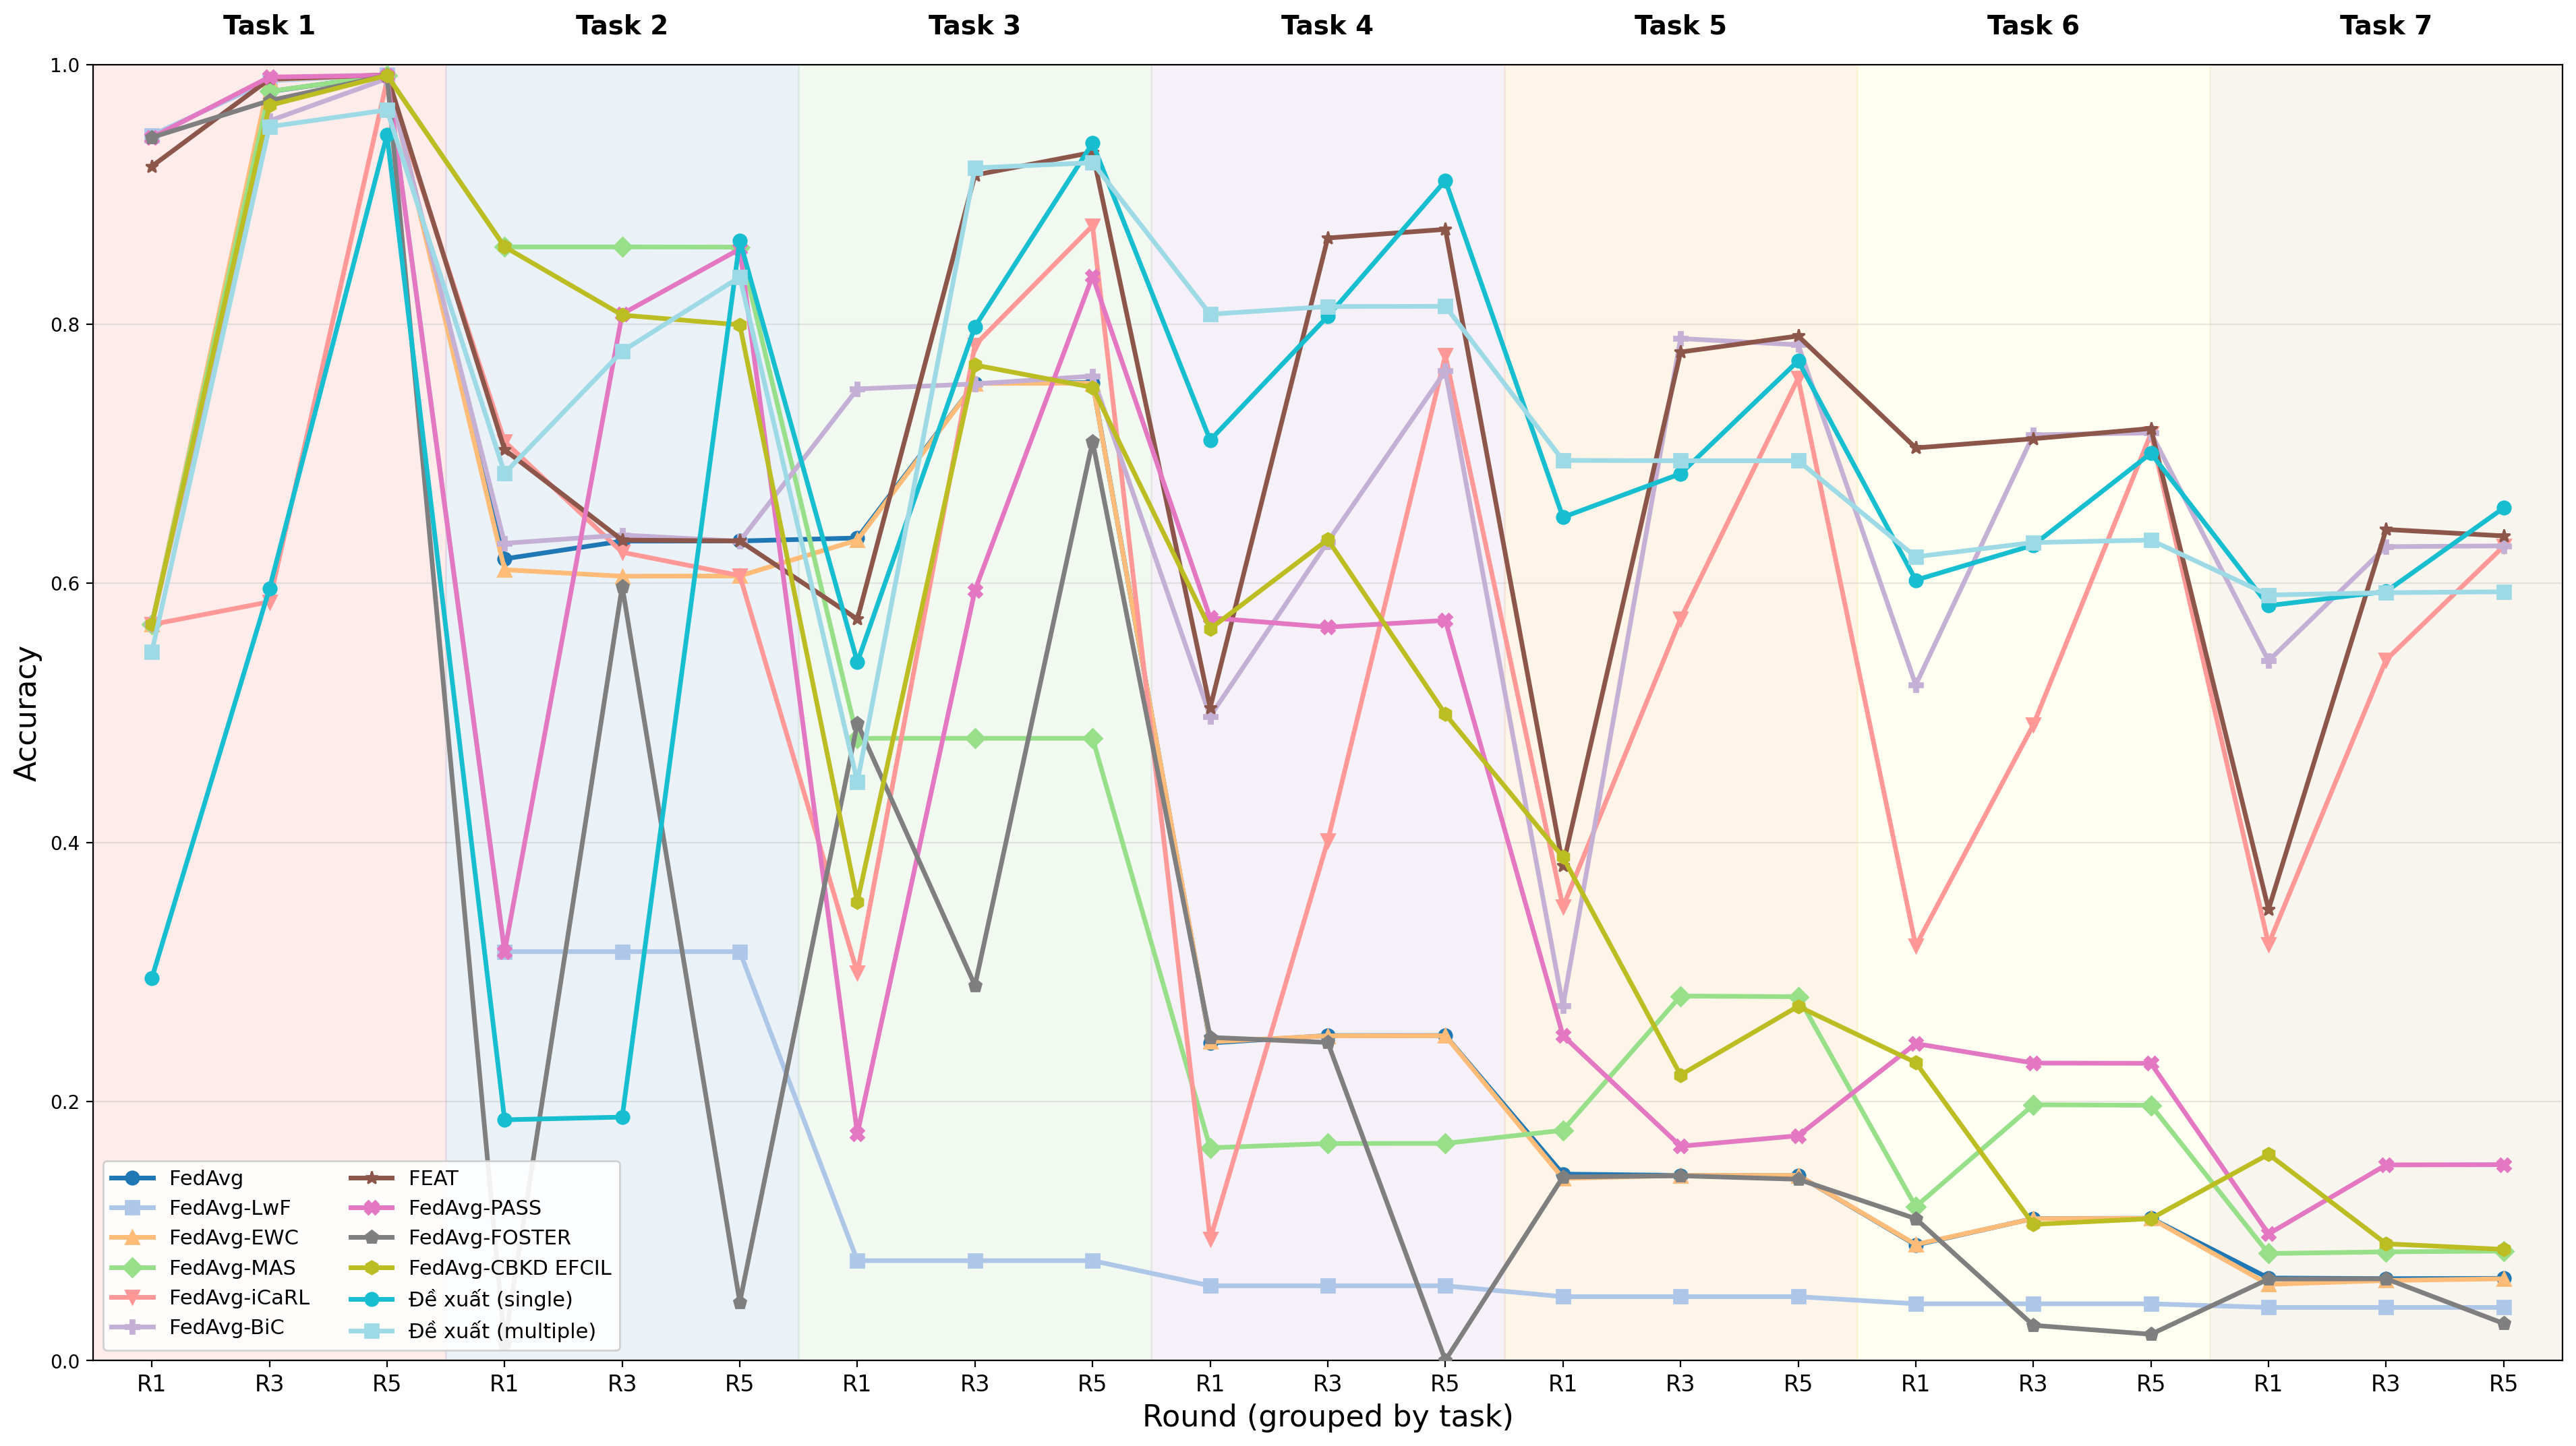
\includegraphics[width=1.0\textwidth]{images/OR_acc.png}
    \caption{Accuracy qua từng vòng liên kết của các phương pháp}
\label{fig:or_acc}
\end{figure*}

\begin{figure*}[ht]
    \centering
    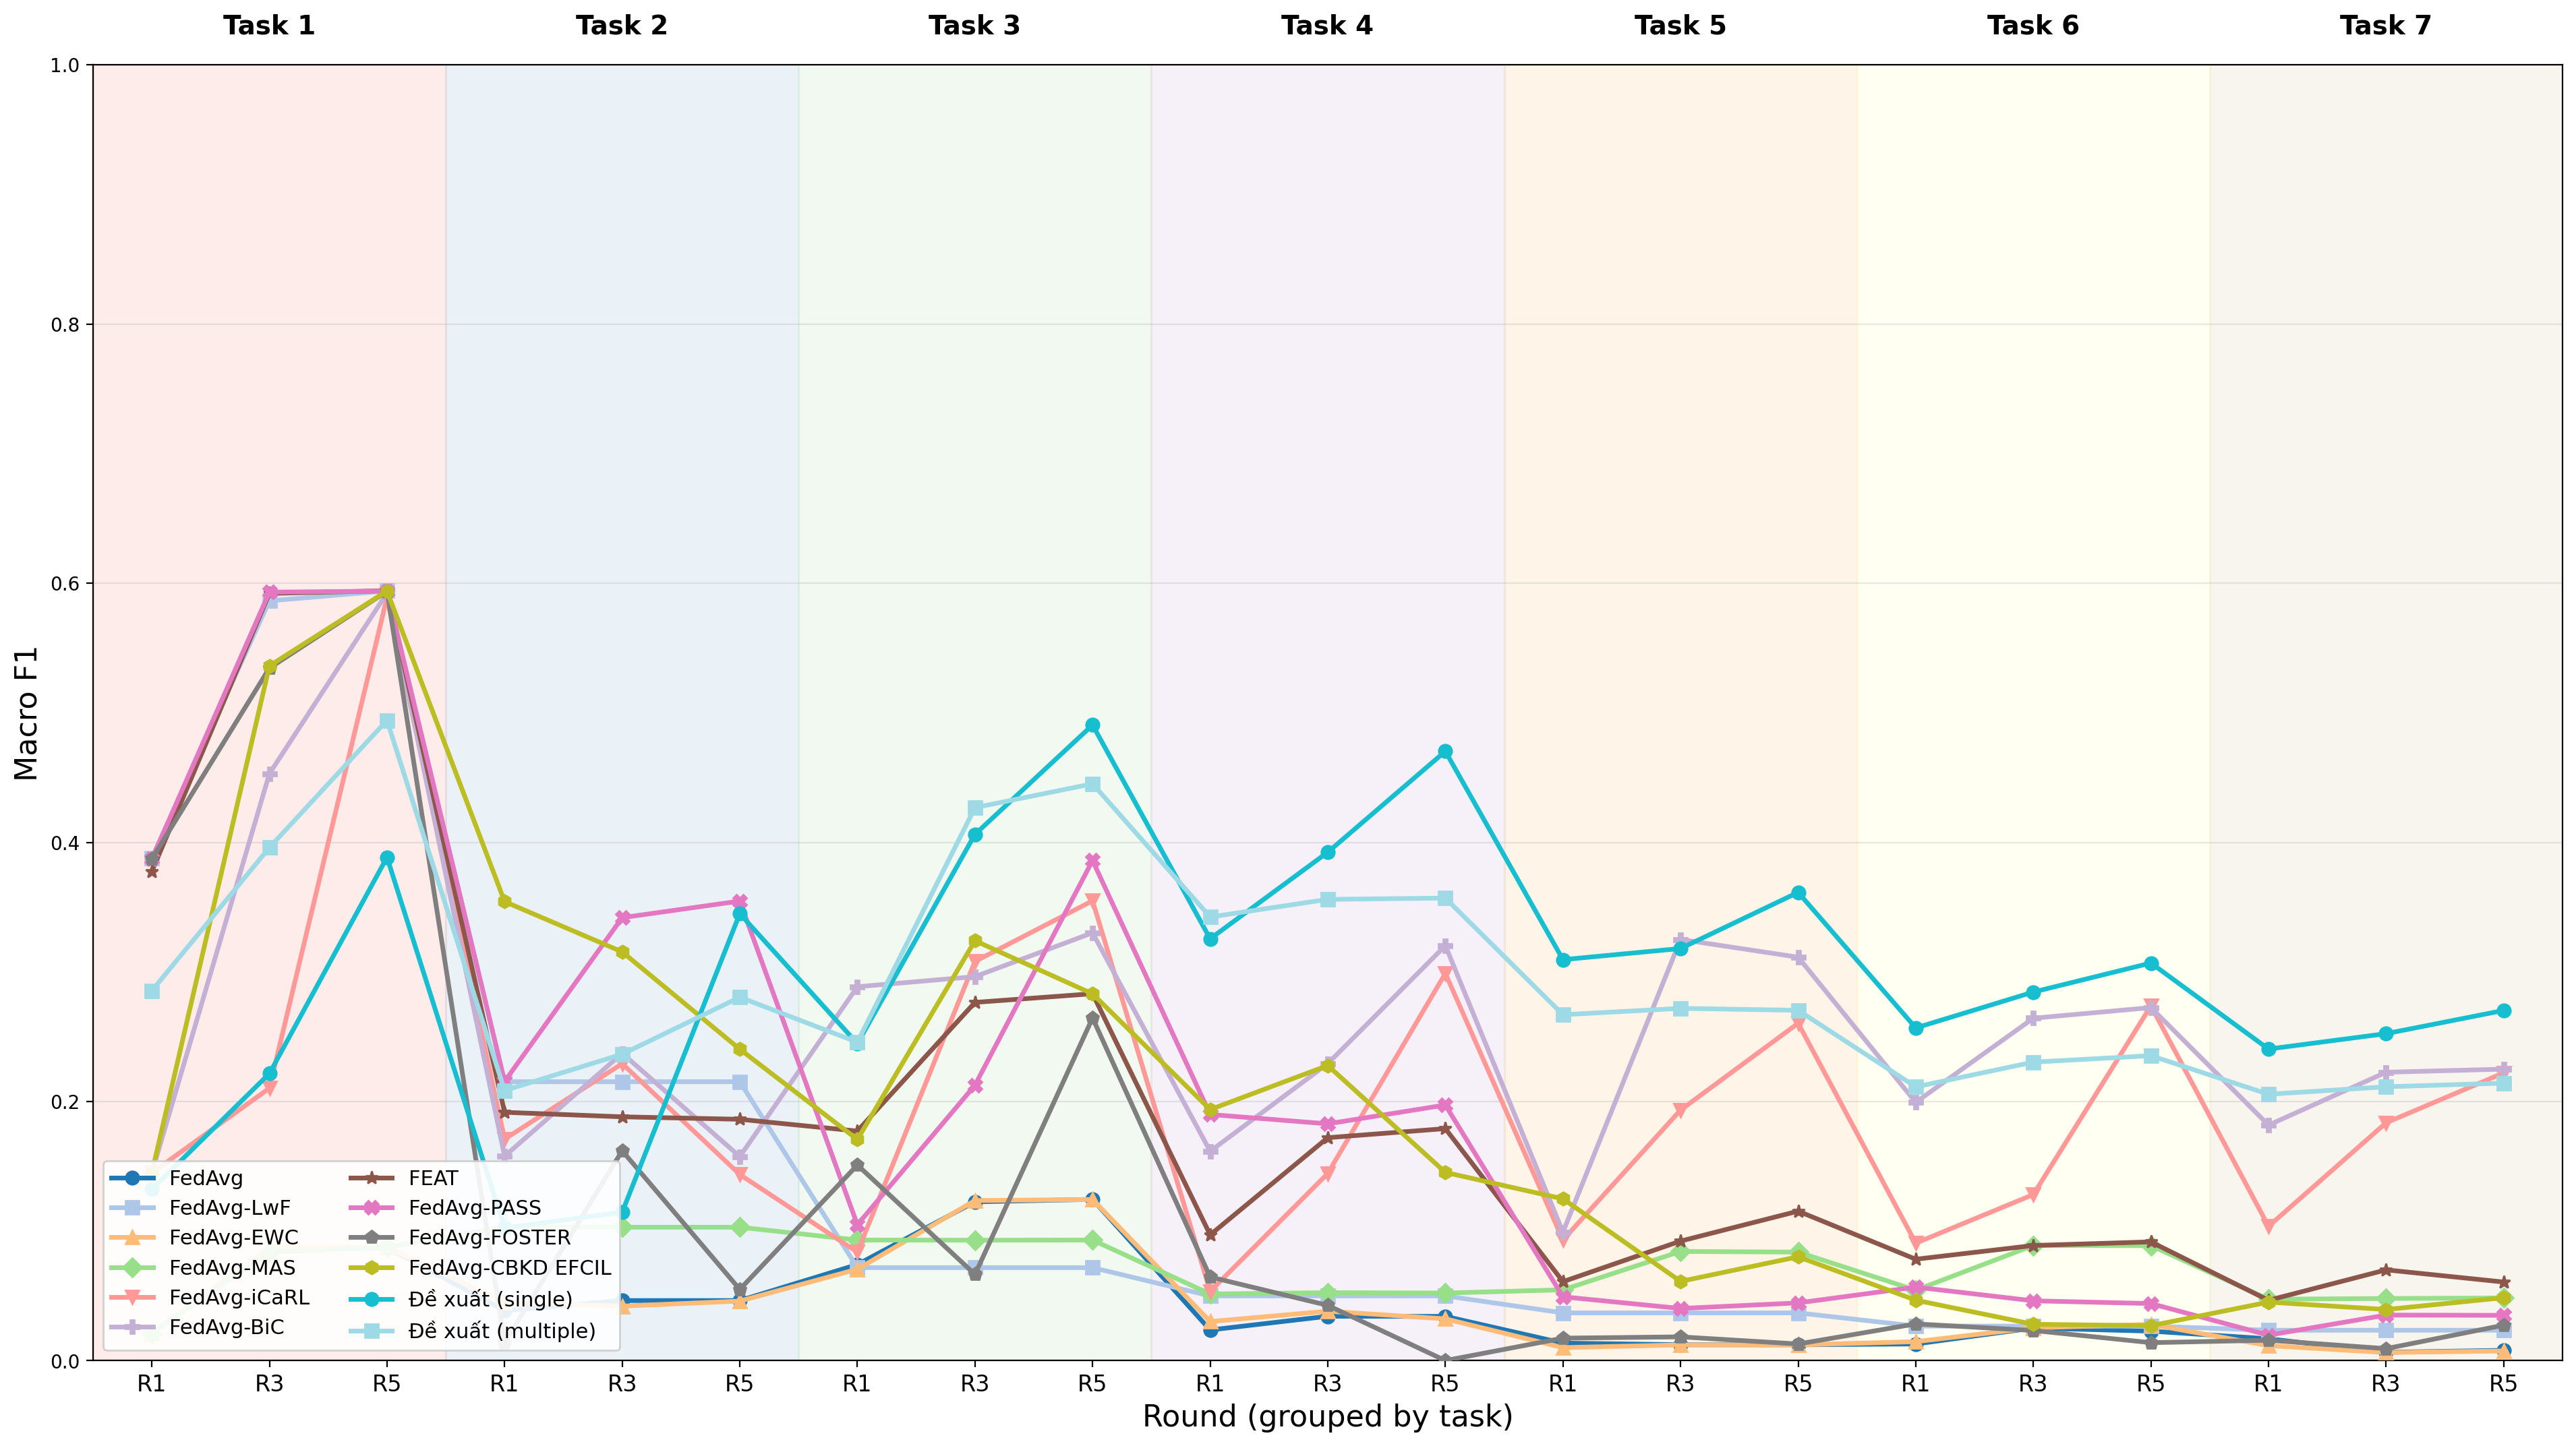
\includegraphics[width=1.0\textwidth]{images/OR_mf1.png}
    \caption{Macro F1 qua từng vòng liên kết của các phương pháp}
\label{fig:or_macf1}
\end{figure*}

\begin{figure*}[ht]
    \centering
    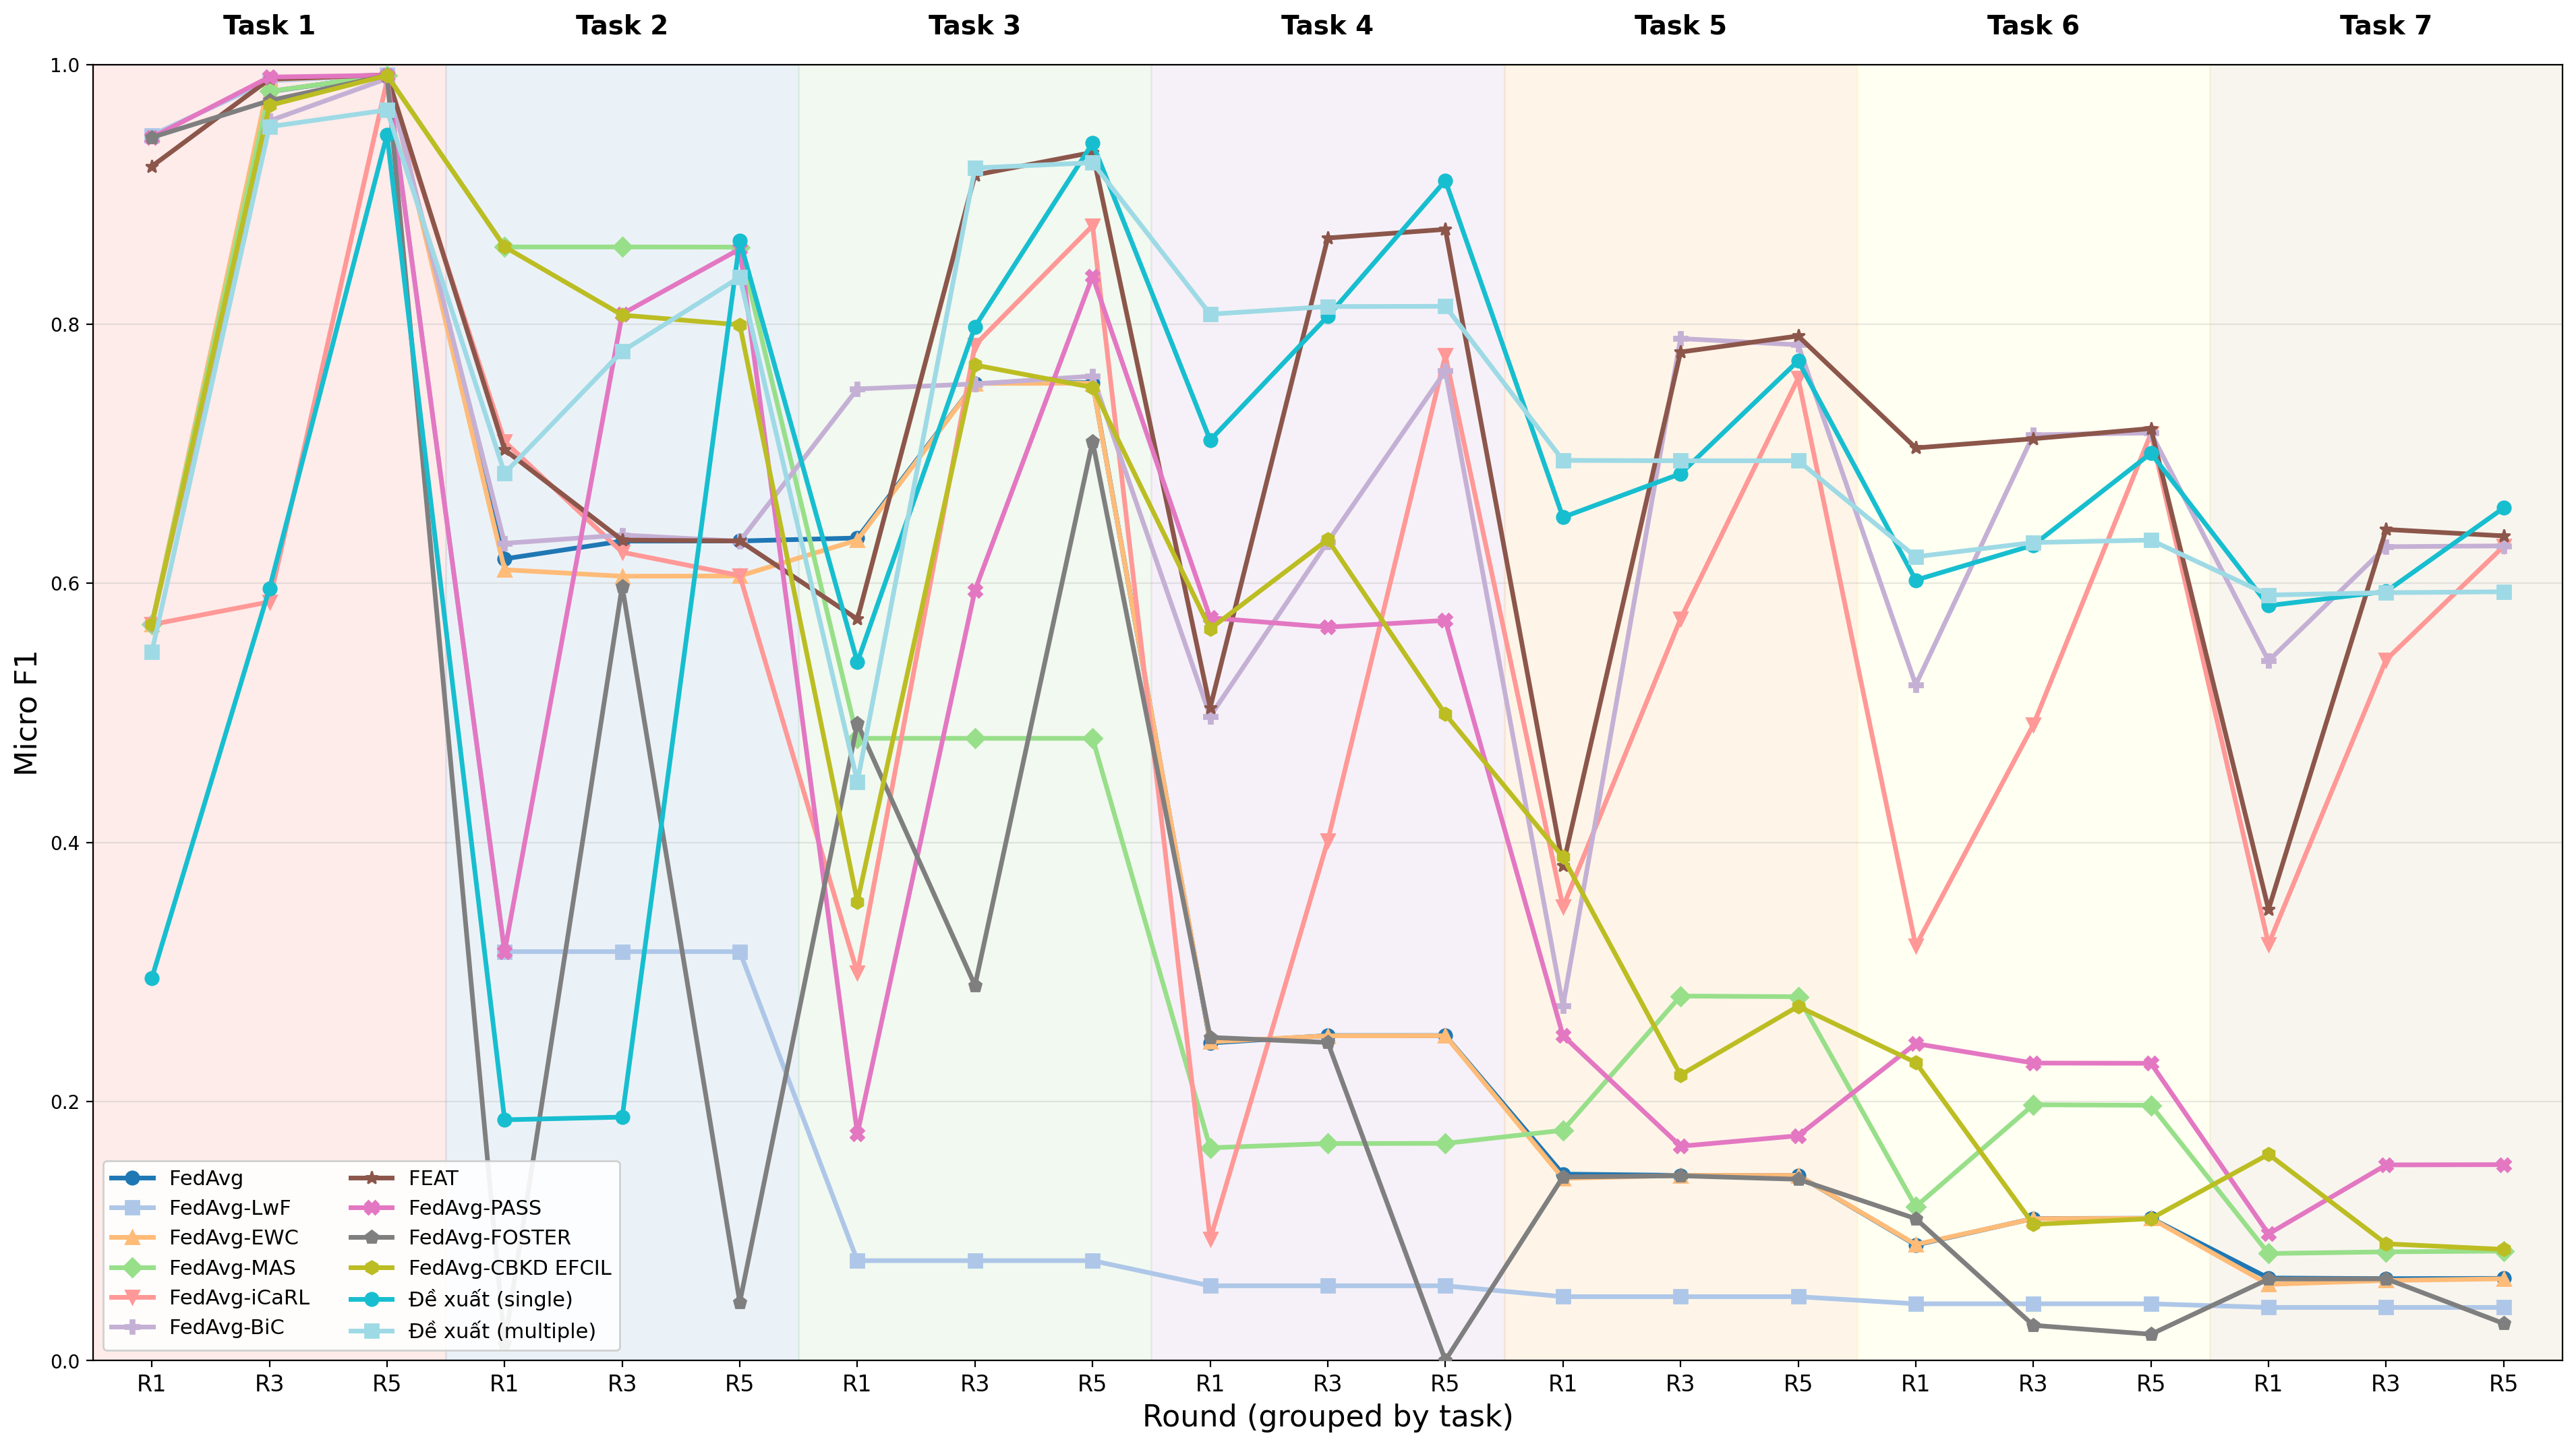
\includegraphics[width=1.0\textwidth]{images/OR_micf1.png}
    \caption{Micro F1 qua từng vòng liên kết của các phương pháp}
\label{fig:or_micf1}
\end{figure*}

\begin{figure*}[ht]
    \centering
    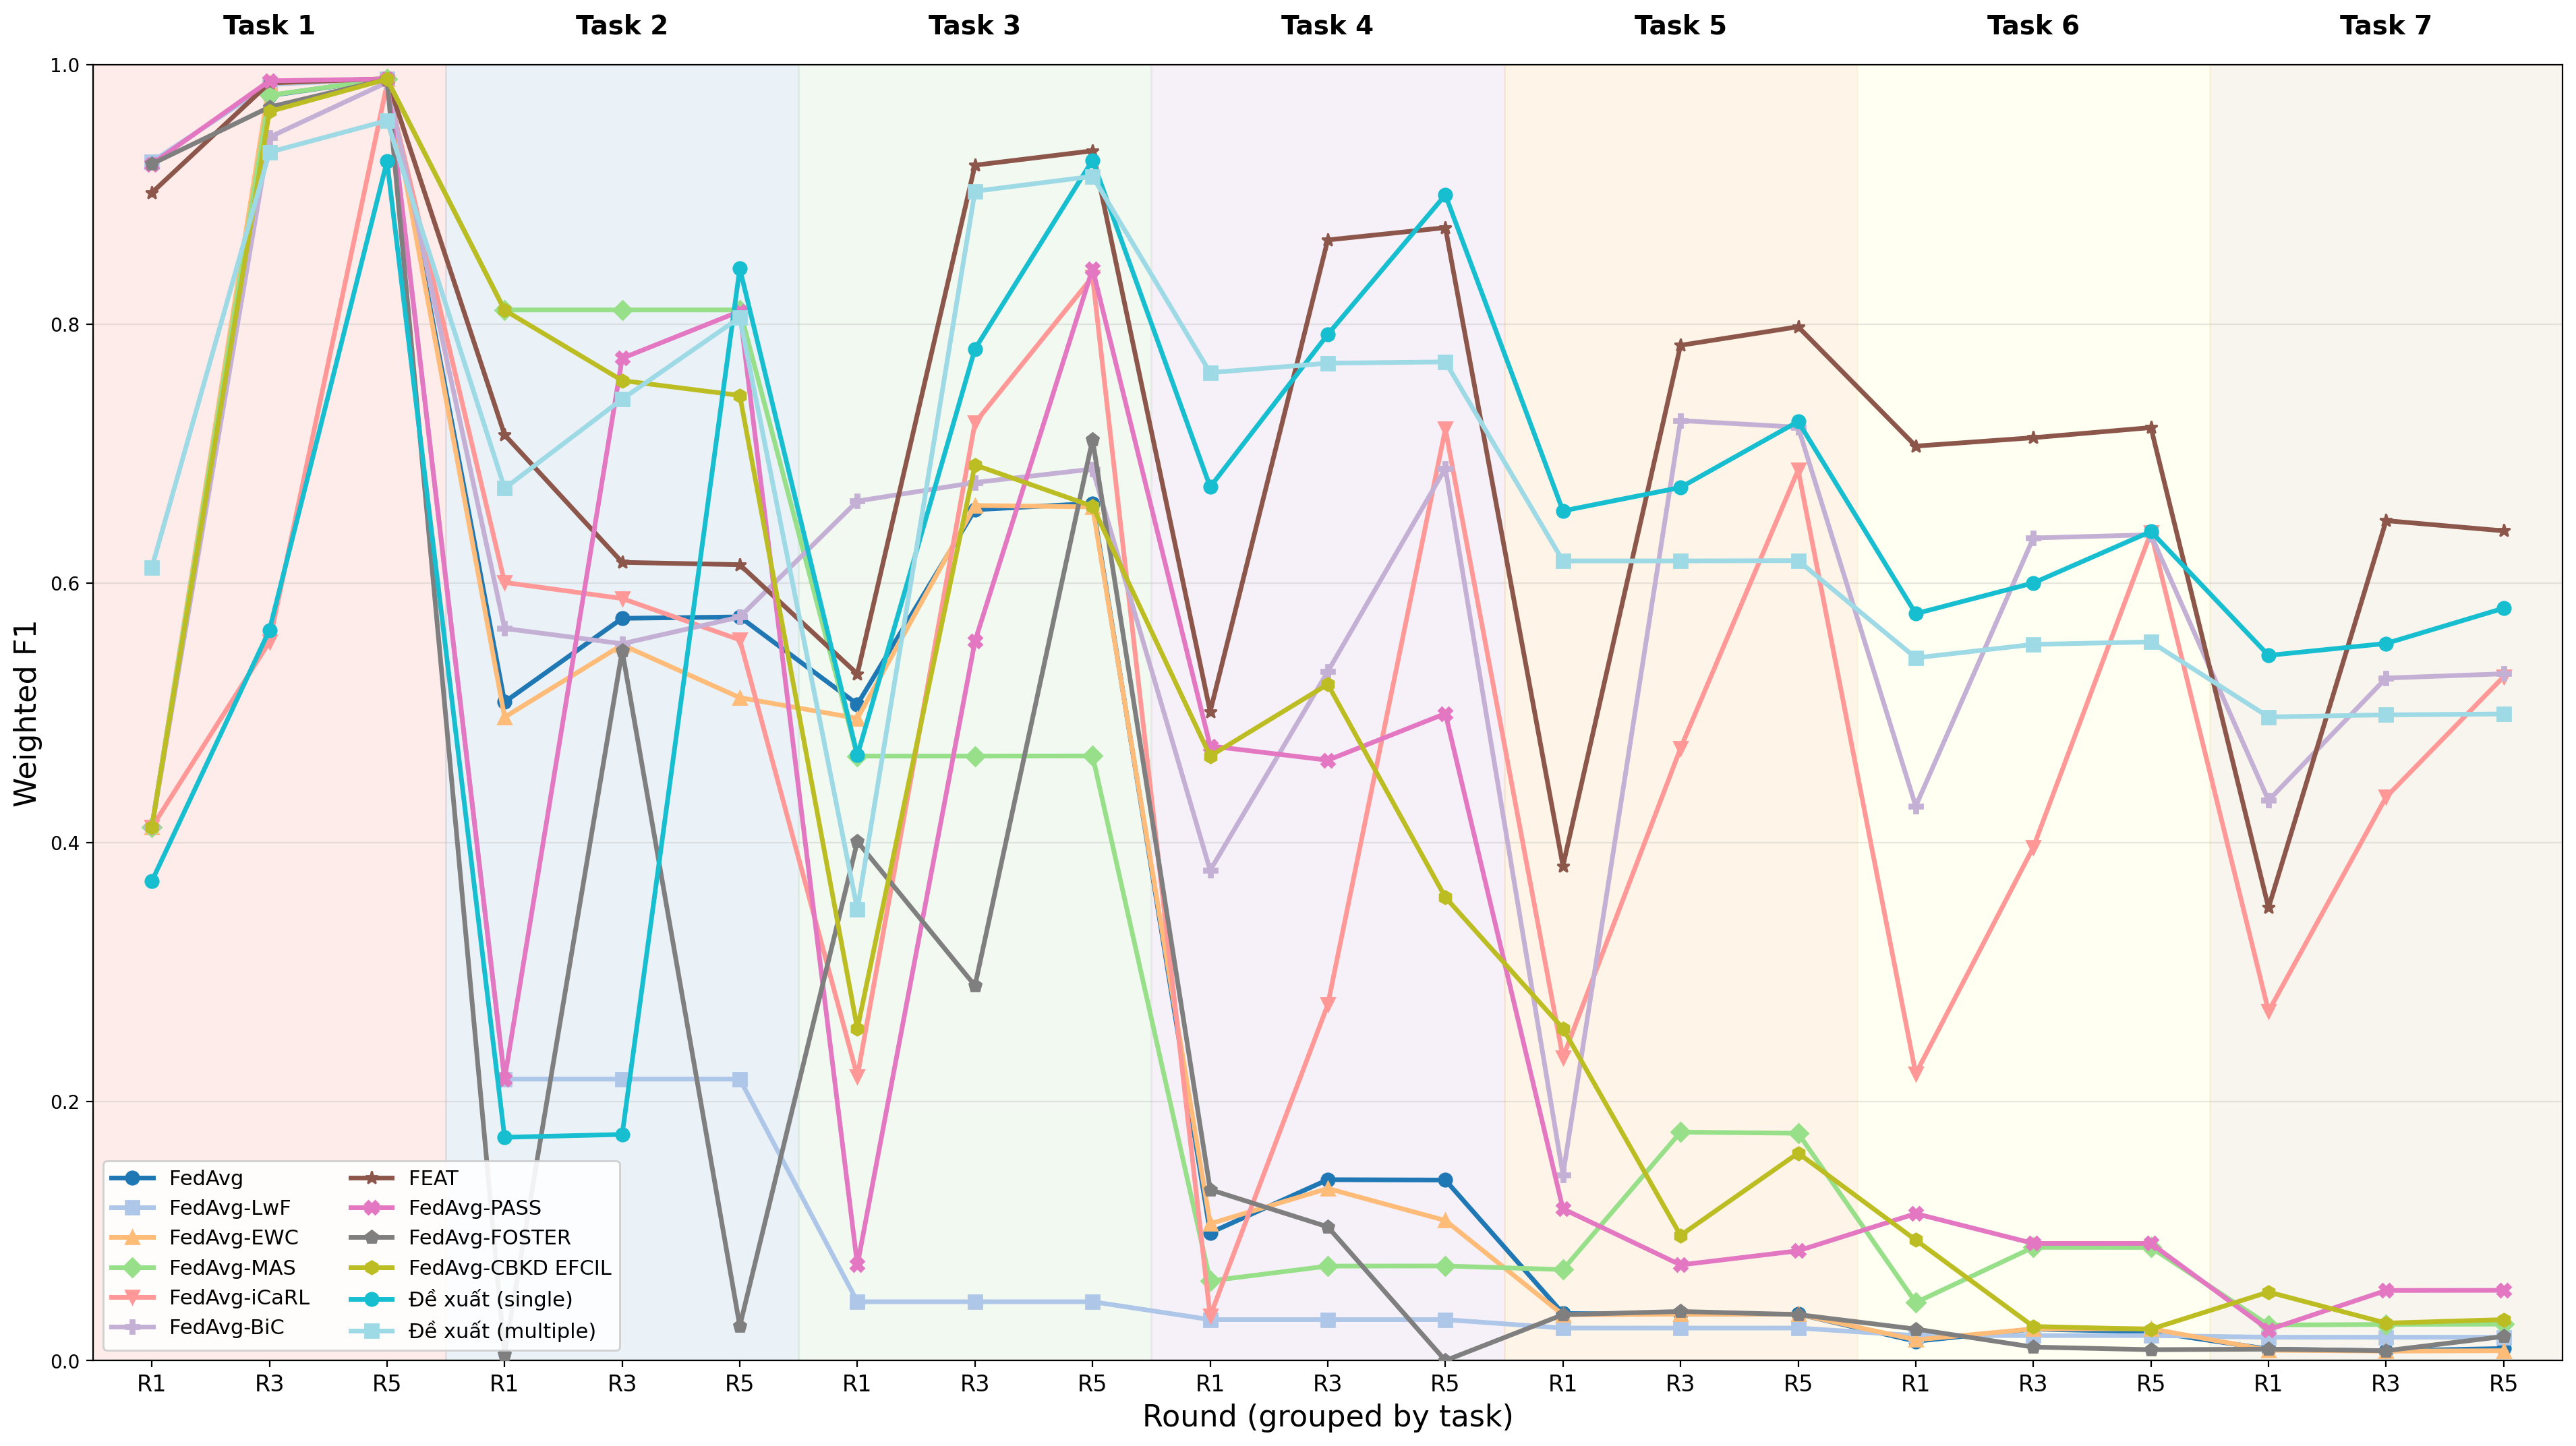
\includegraphics[width=1.0\textwidth]{images/OR_wf1.png}
    \caption{Weighted F1 qua từng vòng liên kết của các phương pháp}
\label{fig:or_wf1}
\end{figure*}

Bảng \ref{tab:cil_config} trình bày cấu hình của các thuật toán học tiệm tiến được đánh giá, bao gồm tham số ràng buộc, số mẫu được sử dụng để học tái diễn, và temperature chắt lọc.

\begin{table}[H]
    \centering
    \caption{Cấu hình các thuật toán học tiệm tiến.}
    \resizebox{\linewidth}{!}{
    \begin{tabular}{lcccc}
        \hline
        Thuật toán & Tham số & Số mẫu & Temperature & Ghi chú \\
        \hline
        FedAvg-EWC        & $\lambda=1000$ & - & - & Regularization \\
        FedAvg-MAS        & $\lambda=200$ & - & - & Regularization \\
        FedAvg-LwF        & $\alpha=0.99$ & - & $T=2$ & Regularization \\
        FedAvg-PASS       & $\lambda=10.0$, $\gamma=10.0$ & 1 \% & - & Prototype augment \\
        FedAvg-CBKD EFCIL & $\lambda=10.0$, $\alpha=10.0$, $\beta=10.0$ & 1 \% & - & Regularization \\
        FedAvg-iCaRL      & - & 1 \% & - & Replay \\
        FedAvg-BiC        & valid $=0.4$ & 1 \% & - & Replay \\
        %FEAT       & $\lambda=1.0$, $\rho=0.9$, $\tau=0.5$ & 1 \% & - & Replay \\
        FedAvg-FOSTER     & $\beta_1=0.97$, $\beta_2=0.97$ & 1 \% & - & Dynamic arch \\
        \hline
    \end{tabular}}
    \label{tab:cil_config}
\end{table}


\subsection{Thảo luận chung}

Chương này đã trình bày toàn bộ quá trình hiện thực và đánh giá phương pháp đề xuất trong môi trường học liên kết tiệm tiến lớp, đồng thời đặt phương pháp này trong tương quan với các hướng tiếp cận tiêu biểu của học tiệm tiến. Xét riêng về độ chính xác phân loại, phương pháp đề xuất chỉ đạt mức xấp xỉ so với các phương pháp replay-based như iCaRL, và sự chênh lệch này phản ánh đánh đổi có chủ đích trong thiết kế: thay vì tối ưu cực đại một chỉ số đơn lẻ, phương pháp hướng đến một tập hợp các tính chất hệ thống vốn ít được giải quyết đồng thời trong các nghiên cứu hiện có về học liên kết tiệm tiến lớp.

Trước hết, phương pháp đề xuất hỗ trợ học liên kết giữa các kiến trúc mô hình khác nhau (model heterogeneity), được được hiện thực (ký hiệu (multiple) trong bảng so sánh \ref{tab:cil_results_task6}) cho phép các client triển khai những mô hình hoàn toàn khác nhau mà vẫn cùng tham gia một quá trình học liên kết thống nhất. Xuyên suốt mọi task, hiệu quả phân loại của kịch bản đa kiến trúc mô hình liên tục tiệm cận các phương pháp đơn cấu trúc và thậm chí thuộc nhóm dẫn đầu ở một số task như task 2 với Accuracy tại task 2 ở $0.9245$, gần tương đương với FEAT ở $0.9325$, một phương pháp State-of-the-art đơn kiến trúc. Phương pháp trong kịch bản này cho thấy chỉ số Macro Precision cao thường xuyên dẫn đầu xuyên suốt 7 task học tiệm tiến. Đây là kết quả thực nghiệm khi có đến $25\%$ số client sử dụng mô hình nhỏ là CNN \ref{tab:cnn_arch}, và các mô hình không chỉ khác nhau về số đối mà còn khác nhau về mặt kiến trúc.

Ở kịch bản đơn kiến trúc, phương pháp đề xuất liên tục dẫn đầu so với các phương pháp khác, và luôn nằm ở mức tương đương so với FEAT. Điều này cho thấy hiệu quả học tiệm tiến rõ rệt của phương pháp đề xuất.

Tuy nhiên khác với FEAT, trong phương pháp đề xuất, do tri thức được trao đổi dưới dạng logits trên tập dữ liệu công khai thay vì trọng số mô hình, hệ thống đề xuất hoàn toàn tránh được các tấn công inference lên trọng số mô hình, giảm thiểu bề mặt của tấn công membership inference và hoàn toàn hỗ trợ được nhiều kiến trúc mô hình khác nhau trong quá trình học liên kết. Cùng với đó, cơ chế trao đổi dựa trên dữ liệu công khai mở ra khả năng triển khai phi tập trung mà không cần một máy chủ tổng hợp tham số trung tâm.

% Cuối cùng, phương pháp đề xuất cho phép điều chỉnh linh hoạt chi phí truyền thông. Bảng \ref{tab:comm_cost_cil} cho thấy các phương pháp dựa trên tham số như FedAvg luôn buộc client phải tải lên toàn bộ trọng số mô hình ở mỗi vòng, nên chi phí truyền thông bị cố định theo kích thước mô hình và không thể co giãn. Ngược lại, vì phương pháp đề xuất trao đổi logits trên dữ liệu công khai, lượng thông tin truyền đi tỉ lệ thuận với số mẫu công khai được chọn, nên người triển khai có thể chủ động đánh đổi giữa băng thông và chất lượng đồng thuận bằng cách điều chỉnh tỉ lệ dữ liệu công khai tham gia trao đổi. Tính co giãn này biến chi phí truyền thông từ một ràng buộc cứng thành một tham số thiết kế có thể tinh chỉnh theo điều kiện hạ tầng cụ thể của từng bên tham gia.

Như vậy, khóa luận này đã thành công trình bày một hệ thống học máy liên kết cho phát hiện xâm nhập có tính ứng dụng thực tiễn cao và đồng thời giải quyết được các khó khăn cũng như điểm yếu của những hệ thống học liên kết truyền thống, với hiệu suất hoạt động cạnh tranh cao với các thuật toán học tiệm tiến hiện đại.